
\section{The James construction} % <<<
\label{TheJamesConstruction}
\ifx\OutputTheJamesConstruction\undefined\else
First, remember the group $J(X)$.  This was the quotient of $KO(X)$ by the equivalence generated on the level of bundles by $V \simeq_J W$ if and only if $S(V \oplus n \varepsilon) \simeq_\textup{f.h.e.} S(W \oplus n \varepsilon)$.  An immediate consequence of the vector field problem is:\footnote{Note that theorem \ref{KOtoJofRPm} is part of theorem \ref{AdamsKORPn} (Adams), and theorem \ref{AdamsKORPn} solves the vector field problem.}
\ConfusedBox{
\textbf{Is this the point?}
Suppose that it is known that $\widetilde{KO}(\RP^m)\simeq\Z/a_m\Z$, and that it is generated by $[\bundle{L}]-1$ (this is the first part of theorem \ref{AdamsKORPn}). Then we can prove the rest of theorem \ref{AdamsKORPn} (i.e.\ theorem \ref{KOtoJofRPm}) using the discussion in lecture \ref{UsingTheSquaresAndThomSpaces}. Recall that theorem \ref{AdamsKORPn} implies the solution of the vector fields problem.
\begin{thm} \label{KOtoJofRPm}
The surjection $\widetilde{KO}(\RP^m) \onto \widetilde J(\RP^m)$ is an isomorphism.
\end{thm}
\begin{proof}
$n(\bundle{L} - 1) \mapsto 0$ means $n \bundle{L}$ is stably fiber homotopy trivial; this implies a (stable) splitting:
\begin{diagram}[height=1.52em]
\RP^{m+n}_n & \rTo & S^n \\
\uTo & \ruTo_\simeq \\
S^n
\end{diagram}
But we know from lecture \ref{UsingTheSquaresAndThomSpaces} that this implies that $\nu(n)\geq m+1$, and since $m\geq \varphi_m$, $a_k=2^{\varphi_m}$ divides $n$, so $n(\bundle{L} - 1)$ was already zero in $\widetilde{KO}(\RP^m)$.\footnote{Homework: compute $\widetilde J(S^n)$.}
\end{proof}
}
Relations to problems in unstable homotopy are often mediated by the EHP sequence, so the next topic will be to construct it.  Our starting point will be a theorem of Bott and Samelson about $H_*(\Loops \Suspend X)$; for a proof see Whitehead~\cite{Whitehead}.  There is a map $\alpha: X \to \Loops \Suspend X$ which embeds $X$ as the ``straight loops'': $\alpha$ is adjoint to $\textup{Id}_{\Sigma X}$, and sends $x\in X$ to the loop $t\mapsto [t,x]$.
%\begin{figure}[h!]
%\centering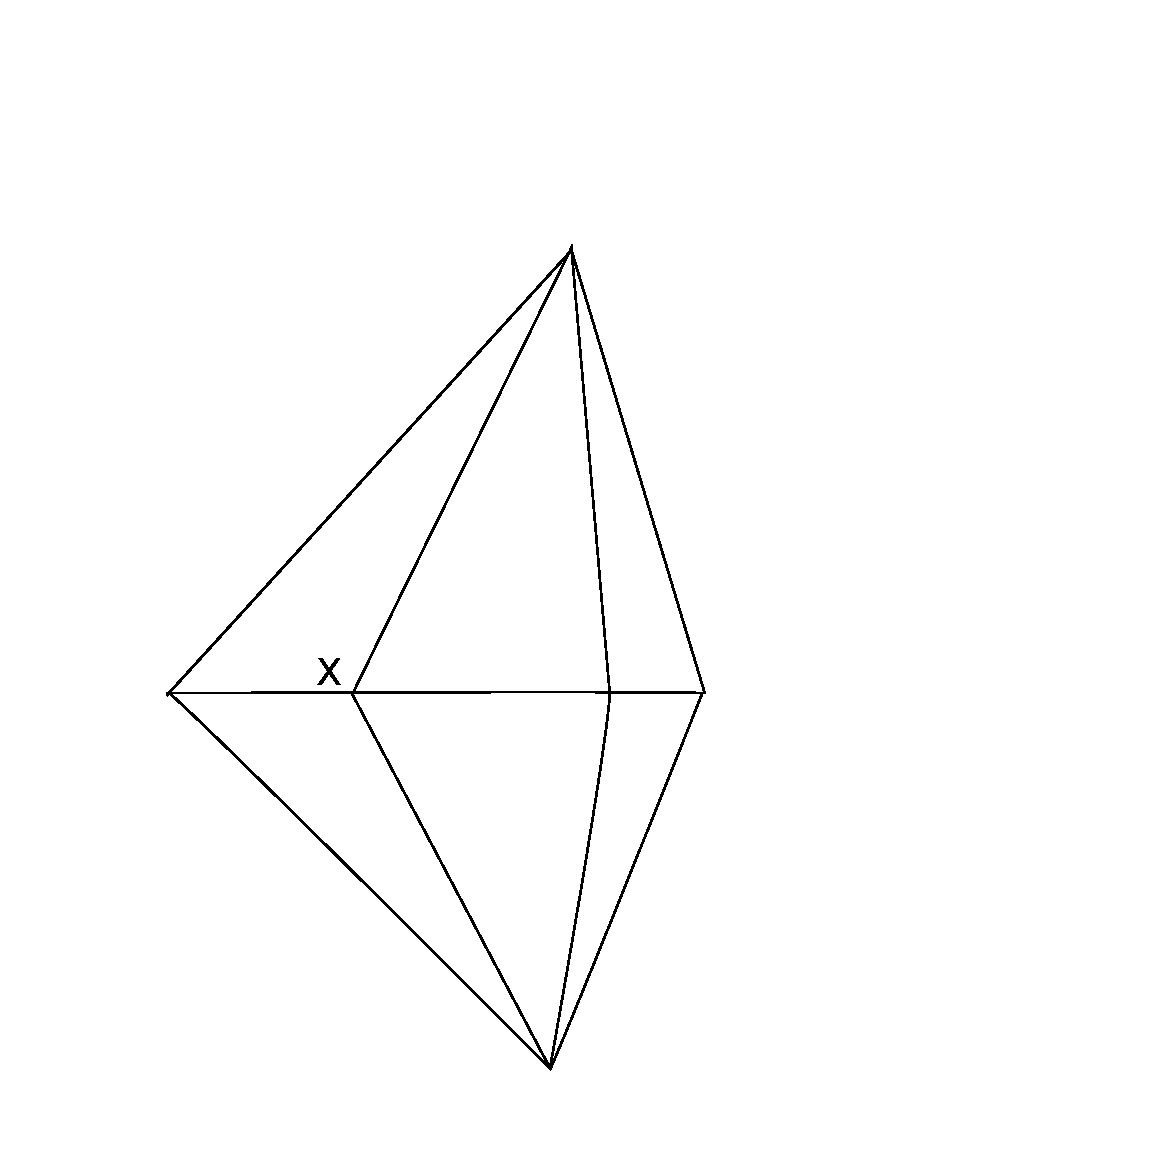
\includegraphics[width=0.3\textwidth]{figures/17.pdf}
%\caption{\small The image of $x$ under $\alpha$.}
%\end{figure}
Choose a coefficient ring $R$.
The loop structure makes $H_* (\Loops \Suspend X)$ into an algebra, so $\alpha_*: \widetilde H_*(X) \to H_* (\Loops \Suspend X)$ yields a unique extension to the tensor algebra $\mathrm{T}(\widetilde H_*(X;R))$ on the $R$-module $\widetilde H_*(X;R)$ (here, tensor products are over $R$):
\[\xymatrix{
\mathrm{T}(\widetilde H_*(X;R))\ar[r]^{\overline\alpha}&H_*(\Omega\Sigma X;R)\\
\ar@{=}[u]\bigoplus_{k\geq0}\widetilde H_*(X;R)^{\otimes k}&
\widetilde H_*(X;R)\ar@{_{(}->}[l]\ar[u]_{\alpha_*}
}\]
\begin{thm}
If $X$ is connected, $R$ is a principal ideal domain, and $H_*(X; R)$ is torsion-free, then $\mathrm{T} (\widetilde H_*(X; R)) \stackrel{\overline \alpha}{\to} H_*(\Loops \Suspend X; R)$ is an isomorphism.
\end{thm}
Now since $H_*(X; R)$ is torsion-free:
\[\bigoplus_{k \ge 0} \widetilde H_*(X;R)^{\otimes k} \cong \bigoplus_{j \ge 0} \widetilde H_* (X^{(k)};R) \cong \widetilde H_*{\left(\textstyle\bigvee_{k \ge 0} X^{(k)};R\right)},\]
so you might hope idealistically that $\Suspend \Loops X$ splits as a wedge of smash powers of $X$.  Of course that's not true, but amazingly enough, it \emph{does} split after one suspension:
\begin{thm}[James, probably]
When $X$ is a connected CW-complex, there is a homotopy equivalence
\[
\Suspend \Loops \Suspend X \simeq \bigvee_{k \ge 1} \Suspend X^{(k)}
.\]
Moreover, this equivalence realises the isomorphism $\overline\alpha$ above.
\end{thm}
\begin{proof}[Proof sketch. \textbf{Come back to this!}]
First, as $X$ is connected, $\Suspend X^{(k)}$ and $\Suspend \Loops \Suspend X$ are simply connected.  If we produce a map giving an isomorphism in homology, then by the Hurewicz theorem we have a weak equivalence.  Then if you believe that both spaces are CW-complexes and some version of the Whitehead theorem, then we're done.

Now, $[\bigvee_{k \ge 1} \Suspend X^{(k)}, \Suspend \Loops \Suspend X]_* = \prod_{k \ge 1}[\Suspend X^{(k)}, \Suspend \Loops \Suspend X]_*$, which is to say that the wedge is the coproduct in the category of pointed spaces and homotopy classes of maps.  So we construct a map on $\Suspend X^{(k)}$ for $k \ge 1$:
\begin{diagram}[height=2em]
\Suspend X^{(k)} & \rTo_{(1)} & \Suspend X^k & \rTo^{\Suspend \alpha^k}_{(2)} & \Suspend(\Loops \Suspend X)^k & \rTo^{\Suspend \mu}_{(3)} & \Suspend \Loops \Suspend X.
\end{diagram}
\begin{enumerate}
\item We've seen this before in the case $k = 2$: we produced a map
\begin{diagram}[height=2em]
\Suspend (X \times Y) & \rTo^{\textup{pinch}} & \Suspend (X \times Y) \wsum & \Suspend(X \times Y) & \rTo^{\Suspend(pr_1 \wsum pr_2)} & \Suspend X \wsum \Suspend Y \\
\uInto & \ruTo_\simeq \\
\Suspend(X \wsum Y).
\end{diagram}
On the other hand the sequence $\Suspend(X \wsum Y) \to \Suspend(X \times Y) \to \Suspend(X \sprod Y)$ combines to provide
\begin{diagram}[height=2em]
\Suspend(X \wsum Y) & \rTo & \Suspend(X \times Y) & \rTo & \Suspend(X \sprod Y) \\
\dTo<\simeq & & \dTo & & \dTo<\simeq \\
\Suspend X \wsum \Suspend Y & \rTo & \Suspend(X \sprod Y) \wsum \Suspend X \wsum \Suspend Y & \rTo & \Suspend(X \sprod Y).
\end{diagram}
The two horizontal lines give exact sequences in homotopy, so by the five lemma and assuming $X$ and $Y$ are CW-complexes, we get a map going back, $\Suspend(X \sprod Y) \wsum \Suspend X \wsum \Suspend Y \to \Suspend (X \times Y)$.  Now the composite $\Suspend(X \sprod Y) \to \Suspend(X \sprod Y) \wsum \Suspend X \wsum \Suspend Y \stackrel{\simeq}{\to} \Suspend(X \times Y)$ gives the first map $\Suspend X^{(k)} \to \Suspend X^k$ in the overall diagram; from its construction we see that it splits the homology of $\Suspend X^k$ as a sum $H_* \Suspend X^{(k)} \oplus H_* ((\Suspend X)^{\wsum k})$ \textbf{incorrect expression}.
\item The second map in the overall diagram is the suspension of the ``straight loops'' embedding that spawned this whole discussion, repeated $k$ times.
\item The third map in the overall diagram is the suspension of the loop multiplication map.  Note that loop multiplication is not strictly associative due to parameterization problems, but it is associative up to homotopy.
\end{enumerate}
Now the Bott-Samelson theorem says that the product of these composities as $k$ ranges over the positive integers is an isomorphism in homology.
\end{proof}

Now note that the Bott-Samelson theorem required that $H^*(X; R)$ be torsion-free and $R$ a principal ideal domain.  However, the claim is that this theorem of James holds for arbitrary coefficients, in particular with $\Z$-coefficients; in fact, we have a general proposition:
\begin{lem}
If $X \to Y$ induces an isomorphism on homology $H_*(X; F) \stackrel{\cong}{\to} H_*(Y; F)$ for $F$ either $\Z_p$ or $\Q$, then $H_*(X; \Z) \stackrel{\cong}{\to} H_*(Y; \Z)$.
\end{lem}
\begin{proof}
Use the universal coefficient theorem cleverly many times.  First, for any $p$, $f$ induces a map of long exact sequences induced by the short exact sequence
\begin{diagram}[height=2em]
0 & \rTo & \Z_p & \rTo & \Z_{p^2} & \rTo & \Z_p & \rTo & 0
\end{diagram}
of coefficients. By the five lemma, $H_*(f;\Z_{p^2})$ is an isomorphism. Similarly, using induction on $n$,
\begin{diagram}[height=2em]
0 & \rTo & \Z_{p^n} & \rTo & \Z_{p^{n+1}} & \rTo & \Z_p & \rTo & 0
\end{diagram}
shows that $H_*(f;\Z_{p^n})$ is an isomorphism for all $n$.

Now the limit $\Z_{p^\infty} = \cdots \into \Z_{p^n} \into \Z_{p^{n+1}} \into \cdots = \bigcup \Z_{p^n}$ is called the ``Pr\"ufer group''. As homology commutes with direct limits, $H_*(f;\Z_{p^\infty})$ is an isomorphism.  Finally, as $\Q/\Z \cong \bigoplus \Z_{p^\infty}$, the sum being taken over all primes $p$,\footnote{View the Pr\"ufer group $\Z_{p^\infty}$ as the quotient in the short exact sequence $0 \to \Z \to \Z[1/p] \to \Z[1/p]/\Z \to 0$. Define a map $\Q\to\Z_{p^\infty}$ by $a/b+c/p^d\mapsto c/p^d$ whenever $b$ is coprime to $p$. Now note that the induced map $\Q\to\prod\Z_{p^\infty}$ factors through the inclusion of $\bigoplus\Z_{p^\infty}$, that this factorisation is surjective, and that it has kernel $\Z$.}
we are done.
\end{proof}

Now the proof of the James' Theorem relied on some heavy stuff: Bott-Samelson, the Hurewicz theorem, and the JHC Whitehead theorem.  You may think that's too slick, and you would be right, because we skipped over the ``James construction.''  The biggest difficulties above were caused by the failure of loop composition to associate.  The idea is to replace $\Loops X$ with a homotopy equivalent space, the ``Moore loops,'' where composition \emph{does} associate.

The space of ``Moore loops'' on $X$ is incredibly simple: since scaling caused trouble, don't scale!  A Moore loop is a map $\omega: [0, T] \to X$, $T \ge 0$, with $\omega(0) = \omega(T) = *$.  Loop multiplication of a Moore loop $\omega: [0, T] \to X$ and another Moore loop $\tau: [0, S] \to X$ gives a loop $\tau \cdot \omega: [0, T + S] \to X$.  We'll call this space $\Loops X$ too, for extra confusion.  $\Loops X$ comes with a basepoint $*$, the path of length 0, and then $\Omega X$ has a strictly associative product with a strict unit *.  We get a map $\alpha: X \to \Loops \Suspend X$ in the same way (notice that the old $\Omega X$ embeds in the Moore loops $\Omega X$).

Now this $\alpha$ factors
\begin{diagram}[height=2em]
X & \rTo^\alpha & \Loops \Suspend X \\
& \rdTo(1,1) \ruTo(1,1)_{\tilde \alpha} J(X)
\end{diagram}
through the space\footnote{``J'' for ``James''.} $J(X)$, the ``free monoid'' on $X$:
\[
J(X) = \coprod_{k \ge 0} X^k / \sim,
\]
where $\sim$ is generated by $x \cdot * = x$.  And the ``real'' theorem is:
\begin{thm}
$\tilde \alpha$ is a homotopy equivalence when $X$ is a connected CW complex.
\end{thm}
Notice that this gives a map back, and so a way of constructing maps out of a loop space.  In general, this is hard to do; adjointness is no help for maps \emph{out} of a loop space.  For example, $J(X)$ is filtered by $J_n = \coprod_{j \le n} X^k / \sim$, and we fill out the following commutative diagram with the obvious maps:
\begin{diagram}[height=2em]
X^n & \rTo & J_n(X) & \rTo & J_n(X) / J_{n-1}(X) & \rEqualto & X^n/F_{n-1}X^n \\
    & \rdTo(6,2) &        &      &                     &           & \dEqualto \\
    &      &        &      &                     &           & X^{(n)}.
\end{diagram}
On the other hand, suspending once we get
\begin{diagram}[height=1.5em]
\Suspend X^{(n)} & \rTo & \Suspend \Loops \Suspend X \\
& & \uTo>\simeq \\
\dTo<{\hbox{split map}} & & \Suspend J(X) \\
& & \uTo \\
\Suspend X^n & \rTo & \Suspend J_n(X) & \rTo & \Suspend X^{(n)},
\end{diagram}
so after one suspension $J_n(X)$ splits as $\Suspend J_n(X) \simeq \bigvee_{k \le n} \Suspend X^{(k)}$.

\textbf{Everything above here would like to be rewritten, and re-understood by me.}

Finally, notice that we have a map $\widehat h_m$:
\begin{diagram}[height=2em]
\bigvee_{\!k \ge 0} \Suspend X^{(k)} & \pile{\rTo^{\simeq} \\ \lTo_{\exists}} & \Suspend \Omega \Suspend X \\
\dTo<{\Suspend(\hbox{collapsing})} & \ldTo_{\widehat h_m} \\
\Suspend X^{(m)}.
\end{diagram}
Its adjoint $h_m: \Loops \Suspend X \to \Loops \Suspend X^{(m)}$ is called the ``$m^\textup{th}$ (James-)Hopf invariant.''  If $X = S^n$ and $m = 2$:
\[h_2:\Loops S^{n+1} \to \Loops \Suspend (S^n)^{(2)} = \Loops S^{2n+1}.\]
%; then $h_2$ is a map $\Loops S^{n+1} \to \Loops \Suspend (S^n)^{(2)} = \Loops S^{2n+1}$.
This is a piece of the EHP sequence; the rest comes from taking the homotopy fiber and looking at the homotopy long exact sequence. Now to compute $H_n (\Loops S^{n+1})$, we use Bott-Samelson:
\[H_* (\Loops S^{n+1}) = \mathrm T(\widetilde H_* (S^n)) = \mathrm T[u_n]\text{ \ where $|u_n| = n$. }\]
So $h_2$ induces a map $\mathrm T[u_n] \to \mathrm T[u_{2n}]$ which preserves degrees, so it couldn't be an algebra map.  So we'd better try cohomology.

\ConfusedBox{
The following has become some kind of aside:

Alternatively, to compute $H_n(\Omega S^{n+1})$, you could use the path fibration $\Loops S^{n+1} \to PS^{n+1} \to S^{n+1}$, $(n > 0)$, and the Serre spectral sequence gives... (draw it).

\textit{Note that if you try to remember grading then $u^2 = (-1) u u$ for $u$ odd, so you lose commutativity by trying to remember grading, which is the reverse somehow of the usual situation. \textbf{I don't really get this.}}
}
\begin{thm}\label{ThmAlgStrucLoopsSphere}
With coefficients in a principal ideal domain \textup{\textbf{(should this say `field'?)}}, there are isomorphisms:
\begin{alignat}{2}
H^* (\Loops S^{2n+1}) & \cong \Gamma[x_{2n}]&\qquad&\text{as Hopf algebras}, \label{FirstIsoEqn}\\
H^* (\Loops S^{2n}) & \cong \Lambda[x_{2n-1}] \otimes \Gamma[x_{4n-2}]&&\text{as algebras}, \label{SecondIsoEqn}\\
H_* (\Loops S^{2k}) & \cong H_*( S^{2k-1}) \otimes H_* (\Loops S^{2k-1})&&\text{as coalgebras, not as algebras.}\label{ThirdIsoEqn}
\end{alignat}
Here, $\Gamma$ stands for the divided polynomial algebra.
\end{thm}
We digress a bit to explain this theorem's statement.  First, we always have a diagonal map $\Delta: X \to X \times X$.  Assuming that $X$ is nice enough (or that the coefficients are nice enough), $H_*(X) \otimes H_*(X) \stackrel{\times}{\to} H_*(X \times X)$ is an isomorphism, so there's a map going backwards as well.  We call the composite of $\Delta_*$ with this inverse map a ``coproduct'', denoted $\Delta$:
\[\xymatrix{
H_*(X)\ar[rd]_{\Delta_*}\ar[rr]^{\Delta\qquad} &&H_*(X)\otimes H_*(X)\ar[ld]^\times_\cong\\
&H_*(X\times X)
}\]
The coproduct map $\Delta$, along with the obvious map $H_* (X) \to R= H_* (\ptspace)$ gives $H_* (X)$ the structure of a coalgebra.

What is a coalgebra?  Well, you reverse the diagrams for an algebra; i.e., you have maps $\Delta: C \to C \otimes_R C$ and $\epsilon: C \to R$ satisfying coassociativity, counitality, and cocommutativity, corresponding to the following three diagrams:
\begin{diagram}[height=2em]
C & \rTo^\Delta & C \otimes_R C \\
\dTo<\Delta & & \dTo>{\Delta \otimes 1} \\
C \otimes_R C & \rTo^{1 \otimes \Delta} & C \otimes_R C \otimes_R C,
\end{diagram}
\begin{diagram}[height=2em]
& & C \\
& \ldTo^\cong & \dTo>\Delta & \rdTo^\cong \\
R \otimes_R C & \lTo^{\epsilon \otimes 1} & C \otimes_R C & \rTo^{1 \otimes \epsilon} & C \otimes_R R,
\end{diagram}
\begin{diagram}[height=2em]
C & \rTo^\Delta & C \otimes_R C \\
& \rdTo^\Delta & \dTo>T \\
& & C \otimes_R C.
\end{diagram}
($T$ involves a sign change for a graded cocommutative coalgebra.)

Suppose $X$ is connected, so $H_0( X) = R$, and there's a well-defined class $1$ in $H_0 (X)$.  Then if $x \in H_n(X)$ where $n > 0$, $\Delta x = 1 \otimes a + \cdots + b \otimes 1$, where any omitted terms have positive degree both in the left- and right-hand factor.  It is clear that $a = b = x$ (by counitality).  If $H_p (X)$ vanishes for $p < n$, then $ \Delta x = 1 \otimes x + x \otimes 1$, and $x$ is called ``primitive.''  Note that in dimension zero, well, $\Delta 1 = 1 \otimes 1$.  This property is called ``group-like;'' it should be called ``set-like,'' but nobody does that.\footnote{The reason for this terminology comes from the example $R[G]$; see below.}

If moreover we are looking at $Y=\Loops X$, well, $\Loops X$ is an $H$-space: the map $\mu: \Loops X \times \Loops X \to \Loops X$ satisfies the requirement that the  forllowing two diagrams homotopy commute:\footnote{Some people call this an associative $H$-space.}
\begin{diagram}[height=2em]
\ptspace \times \Loops X & \rTo & \Loops X \times \Loops X & \lTo & \Loops X \times \ptspace \\
& \rdTo & \dTo>\mu & \ldTo \\
& & \Loops X
\end{diagram}
\begin{diagram}[height=2em]
\Loops X \times \Loops X \times \Loops X & \rTo^{1 \times \mu} & \Loops X \times \Loops X \\
\dTo<{\mu \times 1} & & \dTo<\mu \\
\Loops X \times \Loops X & \rTo^\mu & \Loops X
\end{diagram}
Over field coefficients, this induces the diagram
\begin{diagram}[height=2em]
H_* (Y) \otimes H_* (Y) & \rTo^\psi & H_* (Y) \\
\dTo>\cong & \ruTo_{\mu_*} \\
H_*(Y \times Y),
\end{diagram}
where the isomorphism is of coalgebras.  (We omit the proof; you have to think about what the tensor product of coalgebras ought to be.)  The map $\psi$ is called the ``Pontrjagin product''.

What does this mean, though?  It means that $H_* (Y)$ is a Hopf algebra.  So what's a Hopf algebra?  Well, it's a bunch of structure.  We have maps $\eta: R \to H$ and $\mu: H \otimes H \to H$ that give $H$ an algebra structure and maps $\epsilon: H \to R$ and $\Delta: H \to H \otimes H$ that give $H$ a coalgebra structure.  In addition, $\eta$ and $\mu$ are coalgebra maps, so they give commutative diagrams of the form:
\[\xymatrix{
H\otimes H\ar[r]^\mu\ar[d]^{\Delta\otimes\Delta}
\ar@/_2pc/[dd]_(.7){\Delta_{H\otimes H}}
&H\ar[dd]_\Delta\\
H\otimes H\otimes \makebox[0cm][l]{$H\otimes H$}\ar[d]^{1\otimes T\otimes 1}\\
H\otimes H\otimes H\otimes H\ar[r]^{\qquad\mu\otimes\mu}&H\otimes H
}\qquad
\xymatrix{
H\otimes H\ar[r]^\mu\ar[d]^{\epsilon\otimes\epsilon}
\ar@/_1.3pc/[dd]_(.7){\epsilon_{H\otimes H}}
&H\ar[dld]^\epsilon\\
R\otimes R\ar[d]\\R
}\qquad
\xymatrix@C=3mm{
&R\\
R\ar@{=}[ur]\ar[rr]^\eta\ar[d]_\Delta&&H\ar[ul]_\epsilon\ar[d]^\Delta\\
R\otimes R\ar[rr]^{\eta\otimes\eta}&&H\otimes H
}\]
Now you can check that these diagrams commuting implies that $\Delta$ and $\epsilon$ are algebra maps, so the symmetric conditions are equivalent.

Before going on, another important example of a hopf algebra is, for $G$ a group, the group algebra $R[G]$. The elements are the free $R$-module on $G$, and the product is generated by $[g][h] = [gh]$.  The coalgebra structure comes from $\Delta[g] = [g \otimes g]$ and $\epsilon[g] = 1$ for $g \in G$.  Notice that this explains the terminology ``group-like.''  In fact, the set of group-like elements is exactly the generators.  So the coalgebra structure enables us to recover the generators!

Turning to the Bott-Samelson theorem: if $X$ is connected, $R$ is a principal ideal domain, and $H_* (X)$ is torsion-free, then the theorem gave us an algebra isomorphism $\mathrm T (\widetilde H_n(X))  \cong H_* (\Loops \Suspend X)$.  Now that we have establed that $H_n (\Loops \Suspend X)$ is in fact a Hopf algebra, the natural question is what the Hopf algebra structure on $\mathrm T (\widetilde H_* (X))$ ought to be in order that the isomorphism is one of Hopf algebras.  In particular, what we need is a coproduct map $\Delta: \mathrm T \to \mathrm T \otimes \mathrm T$.  It has to be an algebra map, so by the universality property of $\mathrm T$ all we need is a suitable map $\tilde \Delta: \widetilde H_*(X) \to \mathrm T \otimes \mathrm T$, whose unique extension $\Delta$ is a coproduct map:
\begin{diagram}[height=2em]
\mathrm T (\widetilde H_* (X)) & \rTo^\Delta & \mathrm T (\widetilde H_* (X)) \otimes \mathrm T (\widetilde H_* (X)) \\
\uTo & & \uTo \\
\widetilde H_* (X) & \rTo^{\tilde \Delta} & \widetilde H_* (X) \otimes \widetilde H_* (X),
\end{diagram}
It works out that $\tilde \Delta x$ is the obvious thing. For $x \in \widetilde H_n (X)$, with $n > 0$, $\tilde\Delta$ is defined by:
\[\Delta x = x \otimes 1 + \tilde \Delta x + 1 \otimes x\]


Returning at last to theorem \ref{ThmAlgStrucLoopsSphere}, let's compute the coalgebra structure of $H_* (\Loops S^{n+1}) =\mathrm T[u_n]$:
\begin{alignat*}{2}
\Delta u_n & = u_n \otimes 1 + 1 \otimes u_n,&\qquad&\textup{(as there is no room for middle terms)} \\
\Delta u_n^k & = (u_n \otimes 1 + 1 \otimes u_n)^k,&&\textup{(as $\Delta$ is an algebra map)}
\end{alignat*}
In particular, as the product in $\mathrm T[u_n]\otimes \mathrm T[u_n]$ is $(\mu\otimes\mu)\circ (1\otimes T\otimes1)$, where $T(a\otimes b)=(-1)^{|a||b|}(b\otimes a)$:
\begin{align*}
\Delta u_n^2&=(-1)^{0\cdot n}u_n^2\otimes1+(-1)^{0\cdot0}u_n\otimes u_n+(-1)^{n\cdot n}u_n\otimes u_n+(-1)^{n\cdot 0}\otimes u_n^2\\
&=u_n^2\otimes1+(1+(-1)^{n})(u_n\otimes u_n)+1\otimes u_n^2
\end{align*}
\begin{itemize}
\item When $n$ is even, we could go on to prove that $\Delta u_n^k = {\displaystyle\sum_{i + j = k}} \binom{i+j}{i} u_n^i \otimes u_n^j$.
\item When $n$ is odd, we get that $u_n^2$ is primitive. As $u_n^2$ has even degree:
\begin{align*}
\Delta u_n^{2k} & = \sum_{i+j=k} {\textstyle\binom{i+j}{i}} u_n^{2i} \otimes u_n^{2j}, \text{ \ and}\\
\Delta u_n^{2k+1} & = (\Delta u_n^{2k})(\Delta u_n) \\
& = \sum_{i+j=k} {\textstyle\binom{i+j}{i}} (u_n^{2i+1} \otimes u_n^{2j} + u_n^{2i} \otimes u_n^{2j+1}).
\end{align*}
\end{itemize}
So $H_* (\Loops S^{2k} )\cong H_*( S^{2k-1}) \otimes H_* (\Loops S^{4k-1})$ as coalgebras, though certainly not as algebras giving (\ref{ThirdIsoEqn}).

Now consider $H^* (\Loops S^{n+1})$.  With any coefficients, the group structure is
\[
H^q(\Loops S^{n+1}; R) = \begin{cases} R \langle z_i \rangle & q=ni\textup{ \,(for each $i\geq0$)}, \\ 0 & \mathrm{otherwise}. \end{cases}
\]
Now with field coefficients, let's compute the ring structure.  We can use in this case the pairing of cohomology and homology, so picking $n$ to be even to start, we get
\begin{alignat*}{2}
\langle z_i z_j, u_n^{i+j} \rangle & = \langle \Delta^*(z_i \otimes z_j), u_n^{i+j} \rangle&\qquad& \\
& = \langle z_i \otimes z_j, \Delta_* u_n^{i+j} \rangle \\
& = \left\langle z_i \otimes z_j, \sum_{i'+j'=i+j} {\textstyle\binom{i'+j'}{i'}} u_n^{i'} \otimes u_n^{j'} \right\rangle&&\text{\ (as $n$ is even)} \\
& = {\textstyle\binom{i+j}{i}} = \left\langle {\textstyle\binom{i+j}{i}} z_{i+j}, u_n^{i+j} \right\rangle,
\end{alignat*}
In particular, $z_i z_j = \binom{i+j}{i} z_{i+j}$. This algebra is called the divided polynomial algebra on $z_1$, denoted $\Gamma[z_1]$, and we get $H^* (\Loops S^{2k+1}) \cong \Gamma[x_{2k}]$ as Hopf algebras, which is (\ref{FirstIsoEqn}).

Similarly, the pairing for the odd case gives (\ref{SecondIsoEqn}):
\begin{align*}
H^* (\Loops S^{2k}) & \cong H^* (S^{2k-1}) \otimes H^* (\Loops S^{4k-1}) \\
& \cong \Lambda[x_{2k-1}] \otimes \Gamma[x_{4k-2}],
\end{align*}
but now since the homology isomorphism was only one of coalgebras, this is only an isomorphism of algebras.

% >>>
\fi
\BoxedNote{
Let $X$ be a connected CW-complex, and $X\stackrel{\alpha}{\to} \Omega\Sigma X$ be the inclusion of $X$ as the straight loops of length one in the space of Moore loops on $X$.

\Bullet If $R$ is a PID, and $H_*(X; R)$ is torsion-free, then $\alpha$ induces an isomorphism $\mathrm{T} (\widetilde H_*(X; R)) \stackrel{\overline \alpha}{\to} H_*(\Loops \Suspend X; R)$.

\Bullet There is an equivalence
$\Suspend \Loops \Suspend X \simeq \bigvee_{\!k \ge 1} \Suspend X^{(k)}$ which realises $\overline\alpha$.

\Bullet The extension of $\alpha$ to $J(X)\stackrel{\tilde\alpha}{\to}\Omega\Sigma X$ is a homotopy equivalence. $\Sigma J(X)$ splits as $\bigvee_{\!k \ge 1} \Suspend X^{(k)}$. We define the $m^\text{th}$ James-Hopf invariant $h_m$ via:
\[\widehat h_m:\left\{\Sigma\Omega\Sigma X\to{\textstyle\bigvee_{\!k \ge 0}} \Suspend X^{(k)}\to\Sigma X^{(m)}\right\}\text{ with adjoint }h_m:\Omega\Sigma X\to\Omega\Sigma X^{(m)}\]

\Bullet When $n$ is even, the Hopf algebra $H_*(\Omega S^{n+1})$ is the tensor algebra $\mathrm T[u_n]$, with comultiplication given by $\Delta u_n^k = {\displaystyle\sum_{i + j = k}} \binom{i+j}{i} u_n^i \otimes u_n^j$.

\Bullet With PID coefficients, there are isomorphisms:
\begin{alignat*}{2}
H^* (\Loops S^{2n+1}) & \cong \Gamma[x_{2n}]&\qquad&\text{as Hopf algebras}, \\
H^* (\Loops S^{2n}) & \cong \Lambda[x_{2n-1}] \otimes \Gamma[x_{4n-2}]&&\text{as algebras}, \\
H_* (\Loops S^{2k}) & \cong H_*( S^{2k-1}) \otimes H_* (\Loops S^{2k-1})&&\text{as coalgebras, not as algebras.}
\end{alignat*}
}

\section{The maps \texorpdfstring{$e$ and $h$}{e and h} in the EHP long exact sequence} % <<<
\label{TheMapsEandHinTheEHPLES}
\ifx\OutputTheMapsEandHinTheEHPLES\undefined\else
The march to the EHP sequence continues.
\ConfusedBox{
\textbf{Keep?} Recall for a connected CW complex $X$ the James construction gave a homotopy equivalence
\[
\bigvee_{k \ge 0} \Suspend X^{(k)} \stackrel{\simeq}{\to} \Suspend \Loops \Suspend X
,\]
so in particular we have a map going back.  The map
\[
\bigvee_{k \ge 0} \Suspend X^{(k)} \to \Suspend X^{(m)}
\]
given by smashing everything else to a point gives a composite
\begin{diagram}
\bigvee_{k \ge 0} \Suspend X^{(k)} & \pile{\lTo^\simeq \\ \rTo_{\hbox{Bott-Samelson-James}}} & \Suspend \Loops \Suspend X \\
\dTo & \ldTo_{\hat h_m} \\
\Suspend X^{(m)}
\end{diagram}
whose adjoint $h_m: \Loops \Suspend X \to \Loops \Suspend X^{(m)}$ is the ``$m^\textup{th}$ James-Hopf invariant.''}
Applying the James-Hopf invariant construction when $X = S^n$ and $m = 2$ gives a map $h_2: \Loops S^{n+1} \to \Loops S^{2n+1}$.  The EHP sequence comes from the long exact sequence of the homotopy we get from taking the homotopy fiber of this map.  To start finding out the fiber, we computed the cohomology algebra of $\Loops S^{n+1}$:
\[
H^* (\Loops S^{n+1}) = \begin{cases} \Lambda[x_1] \otimes \Gamma[x_2] & \hbox{when $n$ is odd}, \\ \Gamma[x_1] & \hbox{when $n$ is even}, \end{cases}\textup{\ \ (where $|x_i| = ni$).}
\]


Now the adjoint of the James-Hopf map factors:
\begin{diagram}
\Suspend \Loops S^{n+1} & \rTo^{\hat h_2} & S^{2n+1} \\
& \rdTo(1,1)_{\Suspend h_2} \ruTo(1,1)_\beta \Suspend \Loops S^{2n+1},
\end{diagram}
which is just the expression of adjointness\footnote{%
Here, suppose that $F:\mathscr{D}\longleftrightarrow\mathscr{C}:G$ is an adjunction, that $X\in \mathscr{D}$ and $Y\in\mathscr{C}$, and that $\hat h:X\to GY$ and $h:FX\to Y$ are adjoint. The commuting diagram on the left induces the other commuting diagram, by naturality of the Hom-set isomorphisms:
\[\xymatrix@R=2em{
\ar[d]_{\hat h}X\ar[r]_{\hat h}&GY\ar[d]^{G(\text{Id}_Y)}\\
GY\ar[r]^{\text{Id}}&GY
}
\raisebox{-1.7em}{\textup{\qquad induces\qquad}}
\xymatrix@R=2em{
\ar[d]_{F(\hat h)}FX\ar[r]_{h}&G\ar[d]^{\text{Id}}\\
FGY\ar[r]^{\ \ \hat{\text{Id}}=\text{`$\beta$'}}&Y
}\]
} between $\Loops$ and $\Suspend$.
 $\hat h_2$ came from a splitting, so it splits:
\begin{diagram}[height=2em]
S^{2n+1} & \rTo^{\simeq \hbox{\,Id\ \ \ }} & S^{2n+1} \\
\dInto & & \uTo>{\hat h_2} \\
\bigvee_{\!k \ge 0} \Suspend (S^n)^{(k)} & \rTo^{\hbox{James}} & \Suspend \Loops S^{n+1}.
\end{diagram}
Thus $\hat h_2$ is surjective in homology. As $H_{2n+1}(\Sigma\Omega S^{2n+1})\cong\Z$, the surjective map $H_{2n+1}(\hat h_2):\Z\to\Z$ must be an isomorphism. Then the universal coefficients theorem shows that $H^{2n+1}(\hat h_2)$ is an isomorphism.\footnote{Recall that the reduced homology of $\Sigma\Omega S^{n+1}$ consists of a copy of $\Z$ in degrees $n+1$, $2n+1$, $3n+1$, etc.} In particular, $H^{2n+1}(\Suspend h_2)$ is an isomorphism, so that $H^{2n}( h_2)$ is an isomorphism.
To finish computing the map on cohomology induced by $h_2:\Omega S^{n+1}\to \Omega S^{2n+1}$, there are two cases:
\begin{itemize}
\item First, assume $n$ to be odd. Then $x_1\mapsto u_2$ under $h_2^*$:
\[\xymatrix@R=.5em{
\ar@{=}[d]H^*(\Omega S^{n+1})&H^*(\Omega S^{2n+1})\ar[l]_{h_2^*}\ar@{=}[d]\\
\Lambda[u_1] \otimes \Gamma[u_2]&\Gamma[x_1]\ar[l]
}
\raisebox{-1em}{\ \ where:\ \ }
\xymatrix@R=.5em{
|x_1|=2n,\makebox[0cm][l]{ and }\\
|u_i|=ni.
}
%\xymatrix{u_2&x_1\ar@{|->}[l]}
\]
As $h_2^*$ is an algebra map, $k!x_k = x_1^k \mapsto u_2^k = k! u_{2k}$, hence $h_2^*: x_k \mapsto u_{2k}$.  %In this case $H^* \Loops S^{n+1} = \Lambda[u_1] \otimes \Gamma[u_2]$, so we should study the fate of $u_1$ in the
A simple argument (see claim \ref{SerreSSEHPfiberArg}) using the Serre spectral sequence of the homotopy fibration $F \to \Loops S^{n+1} \to \Loops S^{2n+1}$
%Moreover there can't be anything else in the fiber, because such a thing couldn't survive to $E_\infty$, but on the other hand isn't allowed to hit anything.
shows that $H^*(F; \Z) = \Lambda[u_1]$ with $|u_1| = n$. That is, $F$ has the same cohomology algebra as $S^n$. On the other other hand, we have a map $\alpha: S^n \to \Loops S^{n+1}$ (the map from the Bott-Samelson theorem).  We produce the diagram
\[\xymatrix{
&S^n\ar[dr]^{\text{null}}\ar@{-->}[ld]_\gamma\ar[d]^\alpha\\
F\ar[r]^{j\ \ }&\Omega S^{n+1}\ar[r]^{h_2}&\Omega S^{2n+1}
}
\raisebox{-2em}{\qquad where $j^*(u_1)=u_1$ and $\alpha^*(u_1)$ generates $H^n(S^n)$.}
%\raisebox{-2em}{on $H^{n}(\text{---})$:\qquad}
%\xymatrix{
%&\pm1\makebox[0cm][l]{$\,\in\Z\simeq H^n(S^n)$}\\
%\makebox[0cm][r]{$H^n(F)\simeq\Z\ni\,$}\pm1&u_1\ar@{|->}[u]\ar@{|->}[l]
%}\qquad
\]
The rightmost diagonal map is null-homotopic,\footnote{Simply because $\Omega S^{2n+1}$ is $(2n-1)$-connected.} so the dotted map $\gamma$ exists.  Moreover, $\gamma^*$ is an isomorphism in cohomology.  if $n > 1$, then $\pi_1 (F) = 0$ and $\gamma$ is a homotopy equivalence by the Whitehead theorem.  In case $n = 1$, the long exact homotopy sequence shows $\pi_1 (F) \cong \pi_1 (\Loops S^2) = \Z$, so $\gamma$ is an isomorphism on $\pi_1$.  Now $\gamma$ lifts to a map of universal covering spaces
\begin{diagram}[height=2em]
\widetilde F & \rTo^{\tilde \gamma} & \R \\
\dTo & & \dTo>{e^{i \theta}} \\
F & \rTo^\gamma & S^1,
\end{diagram}
which \emph{are} homotopic by the Whitehead theorem; since $\tilde \gamma$ is equivariant with respect to deck transformations, $\gamma: F \to S^1$ is a homotopy equivalence (\textbf{I do not understand this}).  So now for n odd we have the homotopy fibration $S^n \to \Loops S^{n+1} \to \Loops S^{2n+1}$ whose long exact sequence is the EHP sequence
\[
\cdots \to \pi_i (S^n) \stackrel{e}{\to} \pi_{i+1} (S^{n+1}) \stackrel{h}{\to} \pi_{i+1} (S^{2n+1}) \stackrel{p}{\to} \pi_{i-1} (S^n) \stackrel{e}{\to} \pi_i (S^{n+1}) \to \cdots
\]
\item The case when $n$ is even is even more interesting. Then $x_1\mapsto u_2$ under $h_2^*$:
\[\xymatrix@R=.5em{
\ar@{=}[d]H^*(\Omega S^{n+1})&H^*(\Omega S^{2n+1})\ar[l]_{h_2^*}\ar@{=}[d]\\
\Gamma[u_1]&\Gamma[x_1]\ar[l]
}
\raisebox{-1em}{\ \ where:\ \ }
\xymatrix@R=.5em{
|x_1|=2n,\makebox[0cm][l]{ and }\\
|u_1|=n.
}
%\xymatrix{u_2&x_1\ar@{|->}[l]}
\]
Now, however, $u_2$ is not this bottom class of the divided polynomial algebra, so it is no longer true that $u_2^k = k! u_{2k}$; instead,
\[u_2^k=\left(\frac{u_1^2}{2}\right)^k=\frac{(2k)!}{2^k}u_{2k}.\]
This is a pretty awful number, but if we look at the prime $2$ it's not so bad:
\[
\frac{(2k)!}{2^k} = 1 \cdot \frac{2}{2} \cdot 3 \cdot \frac{4}{2} \cdot \cdots \cdot \frac{2k}{2} = k!\cdot(1\cdot3\cdot\ldots\cdot(2k-1))
,\]
so over $\Z_{(2)}$ this is $k!$ times a unit.  So working over $\Z_{(2)}$, $h_2^* : x_k \mapsto (\textup{unit})\cdot u_{2k}$.  So the Serre spectral sequence over $\Z_{(2)}$ looks the same as it did in the odd case, and $H_*(\alpha; \Z_{(2)})$ is an isomorphism.  So $\gamma: S^n \to F$ isn't a homotopy equivalence, but it is an isomorphism on $\pi_*$ localized at 2, by Serre's mod-$\mathscr{C}$ theory.
\begin{thm}
Let $\alpha: X \to Y$ be a map of simply connected spaces.  If $\alpha_*: H_*(X; \Z_{(p)}) \to H_*(Y; \Z_{(p)})$ is an isomorphism, then $\alpha_*: \pi_* (X) \otimes \Z_{(p)} \stackrel{\cong}{\to} \pi_* (Y) \otimes \Z_{(p)}$ is too.
\end{thm}
So for $n$ even, the $2$-local homotopy groups are the same; we have no idea about the unlocalised homotopy groups, but for present purposes we don't care: we get the same EHP sequences for $n$ even, but now localized at 2.
\end{itemize}
\begin{claim}\label{SerreSSEHPfiberArg}
When $n$ is odd, the cohomology of the fiber $F$ of $h_2$ has the same cohomology algebra as $S^n$, and $F\to \Omega S^{n+1}$ is an isomorphism on $H^n$. When $n$ is even, the same holds after localising at $(2)$.
\end{claim}
\begin{proof}
Let $R$ denote $\Z$ when $n$ is odd, and $\Z_{(2)}$ when $n$ is even. We always use coefficients in $R$, and write $E=\Omega S^{n+1}$ and $B=\Omega S^{2n+1}$. Whether $n$ is even or odd, we know that:
\begin{itemize}
\item The cohomology algebra $H^*(E)$ has a copy of $R$ in each degree which is a multiple of $n$.
\item The cohomology algebra $H^*(B)$ has a copy of $R$ in each degree which is a multiple of $2n$, and the map $h_2^*:H^{2kn}(B)\to H^{2kn}(E)$ is an isomorphism (for all $k\in\N$).
\item If $a\in H^{n}(E)$ and $b\in H^{2kn}(E)$ are generators (for any $k\in\N$), then $ab$ generates $H^{(2k+1)n}(E)$.\footnote{If $n$ is odd, $H^*(E)=\Lambda[u_1]\otimes \Gamma[u_2]$, and this is obvious. If $n$ is even, we are using coefficients in $\Z_{(2)}$, and $H^*(E)=\Gamma[u_1]$. We calculate $u_1u_{2k}=\binom{2k+1}{1}u_{2k+1}=(2k+1)u_{2k+1}$, and $2k+1$ is a unit in $\Z_{(2)}$.}
\end{itemize}
%Whether $n$ is even or odd, we know that the cohomology algebra of $E=\Omega S^{n+1}$ has a copy of $R$ in each degree which is a multiple of $n$. We also know that if $a\in H^{n}(E)$ and $b\in H^{2kn}(E)$ are generators (for $k\in\N$), then $ab$ generates $H^{(o+e)n}(E)$.\footnote{If $n$ is odd, $H^*(E)=\Lambda[u_1]\otimes \Gamma[u_2]$, and this is obvious. If $n$ is even, we are using coefficients in $\Z_{(2)}$, and $H^*(E)=\Gamma[u_1]$. We calculate $u_1u_{2k}=\binom{2k+1}{1}u_{2k+1}=(2k+1)u_{2k+1}$, and $2k+1$ is a unit in $s\Z_{(2)}$.} Finally, the cohomology algebra of $B=\Omega S^{2n+1}$ has a copy of $R$ in each degree which is a multiple of $2n$, and we showed above that $H^{2kn}(h_2)$ is an isomorphism for all $k$.

As the maps $H^{2kn}(h_2)$ are isomorphisms, no differentials can ever hit the entries $E^{2kn,0}$ of the associated Serre spectral sequence\footnote{To understand this, consider the edge homomorphism.}, and $E^{2kn,0}_\infty$ is identified isomorphically with $H^{2kn}(E)$.
Thus, the only nonzero $E_\infty$ term with total degree $2kn$ is $E_\infty^{2kn,0}$.

Now no differentials out of the entries $E^{0,j}$ for $j\leq n$ can possibly be nonzero, so that all of the $E_2^{0,j}$ for $j<n$ are zero, and $E_2^{0,n}\simeq R$. Then $E_2^{0,n}=E_\infty^{0,n}$ is identified isomorphically with $H^n(E)$.

Now (for each $k$) we have identified the places where the generators $a\in H^n(E)$ and $b\in H^{2kn}(E)$ appear on the $E_{\infty}$ page --- at $E_\infty^{0,n}$ and $E_\infty^{2kn,0}$ respectively. Thus, the generator $ab\in H^{(2k+1)n}(E)$, must appear in $E_{\infty}^{2kn+i,n-i}$ for some $i\leq n$ (see Subtlety \ref{EinftyProductSubtlety}).
These groups are zero for $i>0$, so that $ab$ appears in $E_{\infty}^{2kn,n}$, which is thus identified isomorphically with $H^{(2k+1)n}(E)$.

Moreover, as $E_2^{2kn,n}\simeq R$ surjects onto $E_\infty^{2kn,n}=R$ as $R$-modules, this map is an isomorphism, so no differentials can ever hit position $E^{2kn,n}$.

% Moreover, the groups $E_\infty^{2kn+r,n-r}$ are zero for $1\leq r\leq n$, so that $E_{\infty}^{2kn,n}$ is identified with a subgroup of $H^{(2k+1)n}(E)$. Thus $E_\infty^{2kn,n}$ is identified isomorphically with $H^{(2k+1)n}(E)$ for each $k$.
%
%OLD: Now that we have identified the places where the generators of $H^n(E)$ and $H^{2kn}(E)$ appear on the $E_{\infty}$ page, we know that the generator of $H^{(2k+1)n}(E)$ must appear in $E_{\infty}^{2kn,n}$. Moreover, the groups $E_\infty^{2kn+r,n-r}$ are zero for $1\leq r\leq n$, so that $E_{\infty}^{2kn,n}$ is identified with a subgroup of $H^{(2k+1)n}(E)$. Thus $E_\infty^{2kn,n}$ is identified isomorphically with $H^{(2k+1)n}(E)$ for each $k$.

To summarise, the groups $E_2^{2kn,0}$ and $E_2^{2kn,n}$ are all equal to $R$, these entries are never hit by any differentials, and never support nonzero differentials, and only these entries are nonzero at $E_\infty$. Thus, none of the $E_2^{0,j}$ can be nonzero except when $j=n$, for if $j$ is chosen minimally amoungst exceptions to this rule, then $E_\infty^{0,j}\neq0$, a contradiction.
%This implies that no differentials out of the entries $E^{0,k}$ for $k<3n-1$ can be nonzero. In particular, all of these groups are zero except for $E_2^{0,n}$, which is a copy of $\Z$.
%
%Now suppose $d^{2n}:E_{2k}^{0,3k-1}\to E_{2k}^{2k,k}$ is nonzero. This differential must be surjective, as otherwise torsion would survive in $E_\infty^{2k,k}$, and  $H^{3k}(E)\simeq\Z$ would have a torsion subgroup, which is absurd.
%%(On the other hand, it would have to be injective, otherwise $E^{0,3k-1}_\infty\neq0$. --- who cares?)
%In particular, the entry $E_2^{0,3k}$ would have to be a copy of $\Z$, which for dimension reasons would survive to $E_\infty$.
%
%At this point we uncover an inconsistency. We know that if $a$ generates $H^n(E)$ and $b$ generates $H^{2n}(E)$, that $ab\neq0$. However, the elements on the $E_\infty$ page corresponding to these elements lie in $E_\infty^{0,n}$ and $E_\infty^{2n,0}$ respectively. Their product lies in $E_\infty^{2n,n}$. However, this group is zero, contradicting the compatibility between multiplication in $H^*(E)$ and on $E_\infty$. Thus, it must be that $E_2^{0,3k-1}=0$.
%
%State why there's nothing in $E_2^{0,3k}$. State that the argument continues ad infinitum.
\end{proof}
\begin{subtlety}\label{EinftyProductSubtlety}
In the Serre spectral sequence, suppose that $x\in E^{s,t}_\infty$ detects $u\in H^{s+t}(E)$ and $y\in E^{p,q}_\infty$ detects $v\in H^{p+q}(E)$. That is, writing $F_sH^{s+t}(E)$ for the $s^\text{th}$ subgroup in the associated decreasing filtration of $H^{s+t}(E)$:
\[u\in F_sH^{s+t}(E)\setminus F_{s+1}H^{s+t}(E)\text{ and }v\in F_pH^{p+q}(E)\setminus F_{p+1}H^{p+q}(E).\]
Then certainly $uv\in F_{s+p}H^{s+p+t+q}(E)$, but it is not necessarily the case that $uv\notin F_{s+p-1}H^{s+p+t+q}(E)$. In particular, $uv$ could be detected on the $E_\infty$ page at any of the positions $E_\infty^{s+p+r,t+q-r}$ for $r\geq0$.
\end{subtlety}

Well now there's lots to do.  Each of these maps has its own personality, so we'll take each in turn.  $e$ is most familiar, so we'll start with it. In fact, $e:\pi_i(S^n)\to\pi_{i+1}(S^{n+1})$ is simply the suspension homomorphism: from the above calculations of $h_2^*$, we see that $e$ is induced by $\alpha:S^n\to \Omega\Sigma S^n$.

You could think of the rest of the maps as the obstruction to $e$ being an isomorphism: since $\pi_{i+1} (S^{2n+1}) = 0$ for $i \le 2n-1$, we have the following excerpts of the EHP sequence:
\begin{diagram}[height=1em]
  &      & \pi_{2n-1} (S^n) & \rOnto^e & \pi_{2n} (S^{n+1}) & \rTo & 0 \\
  &      & \vdots         &          & \vdots \\
0 & \rTo & \pi_i (S^n)      & \rTo^e   & \pi_{i+1} (S^{n+1}) & \rTo & 0,&&\text{($i\leq 2n-2$)}
\end{diagram}
so $e: \pi_i (S^n) \to \pi_{i+1} (S^{n+1})$ is epic if $i = 2n-1$ and an isomorphism if $i < 2n-1$.  This is precisely the statement of the Freudenthal suspension theorem for $S^n$, so the homotopy groups $\pi_k (S^{2n+1})$ and the $h$ and $p$ maps are the obstructions to extending the Freudenthal suspension theorem to higher dimensions.

By the way, earlier we studied the Hopf invariant 1 problem; there were two main results: using $\Sq^n$ we found that if there is an element of Hopf invariant 1 in $\pi_{2n-1} (S^n)$, then $n$ is a power of $2$.
Similarly, we defined a stable version of the Hopf invariant, a homomorphism $\pi_{2n+i-1}(S^{n+i})\to\Z_2$, in which $\Sq^n$ takes the place of the cup square.

Since $\Sq^n$ commutes with suspension, this is a stable result: if $K=S^{n+i}\cup_f e^{2n+i}$ for $f\in\pi_{2n+i-1}(S^{n+i})$, and if $H^{n+i}(K;\Z_2)=\Z_2\langle x\rangle$ and $H^{2n+i}(K;\Z_2)=\Z_2\langle y\rangle$, then $\Sq^n x = y$ implies that $n$ is a power of $2$.  Using $K$-theory we showed that if the (unstable) Hopf invariant is one, then $n$ must be 1, 2, 4, or 8.  This result is not obviously stable from $K$-theory because the Adams operations are not stable.  But now the EHP sequence gives this to us:
\[\pi_{2n-1}(S^n) \stackrel{e^i}{\onto} \pi_{2n-1+i} (S^{n+i})\text{ is surjective},\]
so no new elements are born after suspending any number of times.  This is an example of the EHP sequence taking unstable information and giving back stable information.

Now we move up one row and look at $h$:
\begin{diagram}[height=2em]
\pi_{2n+1} (S^{n+1}) & \rTo^h & \pi_{2n+1} (S^{2n+1}) \simeq \Z%& \rTo^p & \pi_{2n-1} (S^n) & \rTo^e & \pi_{2n} (S^{n+1}).
\end{diagram}
We also have the Hopf invariant $H: \pi_{2n+1} (S^{n+1}) \to \Z$.  To keep them straight, $h$ is the ``James-Hopf invariant'' and $H$ is the ``Hopf Hopf invariant.'' We will show in lemma \ref{HopfisHopfLemma} that the two coincide.
\begin{claim}
If $f:S^{2n+1}\to S^{n+1}$ is an element of $\pi_{2n+1} (S^{n+1})$, then $h(f)=\deg\left\{\hat f:S^{2n}\to\Omega\Sigma S^n\right\}$, where $\hat f$ is the adjoint of $f$, and by $\deg\{\hat f\}$ we mean the degree of $H_{2n}(f):\Z\to\Z$, defined only up to sign.
\end{claim}
\begin{proof}
$h(f)$ is the degree of $\hat q$, the adjoint of the composite
\[q:\xymatrix{
S^{2n}\ar[r]^{\hat f}&\Omega\Sigma S^n\ar[r]^{h_2}&\Omega\Sigma S^{2n}
}\]
Now there are commuting diagrams
\[\xymatrix@C=.2cm{
\Sigma S^{2n}\ar[rr]^{{\hat q}}\ar[rd]_{\Sigma q}&&\Sigma S^{2n}\\
&\Sigma\Omega\Sigma S^{2n}\ar[ru]_{{\epsilon}}
}\qquad
\xymatrix@C=.2cm{
\Sigma\Omega\Sigma S^{n}\ar[rr]^{\Sigma h_2}\ar[rd]_{\hat h_2}&&\Sigma\Omega\Sigma S^{2n}\\
&\Sigma S^{2n}\ar[ru]_{{\eta}}
}\]
From the left diagram,  $h(f)=\deg\hat q=(\deg q)(\deg\epsilon)=\deg q=(\deg\hat f)(\deg h_2)$, where the reader can figure out what we mean each time we write $\deg$. However, from the right diagram, $\deg h_2=\deg\hat h_2=1$ (as $\hat h_2$ is a collapse map). Note that we have used that $\epsilon$ and $\eta$ both have degree one in the appropriate sense.
\end{proof}
\begin{lem}\label{HopfisHopfLemma}
$h(f)=\pm H(f)$ for all $f\in\pi_{2n+1} (S^{n+1})$, so that the names are well-chosen.
\end{lem}
\begin{proof}
We'll calculate $h(f)=\pm H(f)$ for $f\in\pi_{2n+1} (S^{n+1})$. Moreover, we'll write $H$ for $H(f)$ and $h$ for $h(f)$.

First take the case $n$ is even.  Then $H$ is calculated by squaring an odd dimensional cohomology class, so that $H = 0$.
Now let $g$ generate $H_{2n}(S^{2n})$, and write $u_2$ as usual for the generator of $H_{2n}(\Omega S^{n+1})$. By the claim, $\hat f_*(g)=h\cdot u_2$ (up to sign). Now $f_*$ is a coalgebra map, and we have computed the Hopf algebra structure on $H_*(\Omega S^{n+1})=\mathrm{T}[u_n]$, so there is a compatibility:
%\begin{diagram}
%g & \rMapsto^{\hat f_*} & h u_{2n} \\
%\dMapsto & &\rdMapsto>\Delta \\
%g \otimes 1 + 1 \otimes g & \rMapsto & h(u_2 \otimes 1 + 1 \otimes u_2) & \lEqualto u_2 %\otimes 1 + 2 u_1 \otimes u_1 + 1 \otimes u_2.
%\end{diagram}
\[\xymatrix{
g\ar@{|->}[r]_{\hat f_*}\ar@{|->}[d]_{\Delta}&h\cdot u_{2n}\ar@{|->}[dr]^{\Delta}\\
g\otimes1+1\otimes g\ar@{|->}[r]^{\hat f_*\otimes\hat f_*\qquad}&\ar@{=}[r]h\cdot(u_{2n}\otimes1+1\otimes u_{2n})&h\cdot(u_{2n}\otimes1+2u_1\otimes u_1+1\otimes u_{2n})
}\]
But this equality can hold only if $h = 0$, so we are done when $n$ is even.

In the case that $n$ is odd,\footnote{Note that the argument showing that $h = 0$ no longer applies since now $u_2 = u_1^2$ \emph{is} primitive; recall that there is a coalgebra isomorphism $H_* (\Loops S^{2k}) \cong H_* (S^{2k-1}) \otimes H_* (\Loops S^{4k-1})$ in this case.} there are two steps; first we show $h \mid H$, then that $H \mid h$.  To show that $h \mid H$, study these two Barratt-Puppe sequences and the associated exact sequences in cohomology:
\begin{diagram}[height=2em]
S^{2n+1} & \rTo^f & S^{n+1} & \rTo & C(f) & \rTo & S^{2n+2}&\rTo&S^{n+2} \\
\dEqualto & & \uTo>\beta & & \uTo>\chi & & \dEqualto &&\uTo>{\Sigma\beta}\\
S^{2n+1} & \rTo^{\Suspend \hat f} & \Suspend \Loops S^{n+1} & \rTo & \Suspend C(\hat f) & \rTo & S^{2n+2} & \rTo^{\Suspend^2 \hat f} & \Suspend^2 \Loops S^{n+1} \\
%
0 & \lTo^f & \Z & \lTo & \Z\langle x\rangle & \lTo & 0 \\
\makebox[0cm][r]{$H^{n+1}$:\qquad}\dEqualto & & \dTo>{\beta^*}<\simeq & & \dTo & & \dEqualto \\
0 & \lTo^{\Suspend \hat f} & \Z & \lTo & \Z\langle \overline x\rangle & \lTo & 0 &\\
%
 && 0 & \lTo & \Z\langle y\rangle & \lTo & \Z& \lTo & 0 \\
\makebox[0cm][r]{$H^{2n+2}$:\qquad}& & \dTo>{\beta^*} & & \dTo & & \dEqualto &&\dTo\\
&& 0 & \lTo & \Z_h\langle \overline y\rangle & \lTo & \Z & \lTo^{\cdot h} & \Z, \\
\end{diagram}
Now we may choose the generators $\overline x$ and $\overline y$ such that $x\mapsto \overline x$ and $y\mapsto\overline y$. In particular, $x^2=Hy$ then implies that $\overline x^2=H\overline y$. However, as $\Sigma C(\hat f)$ is a suspension,\footnote{Cup products vanish in any cohomology theory on any suspension.} we have $H\overline y=0$, so that $h|H$.

To show that $H \mid h$, we study the map $\Loops k$, where $k$ is the cofiber map $k:S^{n+1}\to C(f)$. We wish to show that $\Omega S^{n+1}\to\Omega C(f)$ induces a map on $H_{2n}$ of the form $\Z\onto\Z_H$. For then, if we look at the Barratt-Puppe sequence:
\[\xymatrix@!0@C=2.5cm@R=1.4cm{
\Omega S^{2n+1}\ar[r]^{\Omega f}&\Omega S^{n+1}\ar[r]&\Omega C(f)\\
S^{2n}\ar[u]^\alpha\ar[ur]^{\hat f}
}
\raisebox{-.6cm}{ on $H_{2n}(\text{---})$: }
\xymatrix@!0@C=2.5cm@R=1.4cm{
\Z\ar[r]^{(\Omega f)_*}&\Z\ar@{->>}[r]&\Z_H\\
\Z\ar[u]^\simeq\ar[ur]^{\hat f_*}_{\cdot h}
}\]
In particular, as the composite $S^{2n}\to \Omega C(f)$ is null, $h\mapsto 0$ under $\Z\onto\Z_H$, so that $H|h$.

% First we want to show that $H_{2n} (\Loops C (f)) = \Z_H$.
In the rational cohomology spectral sequence for the fibration $\Loops C(f) \to PC(f) \to C(f)$, we compute a crucial differential (marked $(\star)$):
\begin{center}
\begin{tikzpicture}
    %Axes
	\path (-1,1.5) node {$\Omega S^{n+1}$};
	\path (+3.5,-.76) node {$S^{n+1}$};
    \draw[->] (-0.2,0) -- (5.25,0);
    \draw[->] (0,-0.2) -- (0,2.5);
    %Horizontal ticks
    \draw (.5,.05) -- (.5,-.05) node[below] {$0$};
    \draw (2.5,.05) -- (2.5,-.05) node[below] {$n+1$};
    \draw (4.5,.05) -- (4.5,-.05) node[below] {$2n+2$};
    %Vertical Ticks
    \draw (.05,.5) -- (-.05,.5) node[left] {$0$};
    \draw (.05,2) -- (-.05,2) node[left] {$n$};
    %Points
    \path (.5,.5) node (v00) {$\Q$};
    \path (2.5,.5) node (v10) {$\Q\langle x\rangle$};
    \path (4.5,.5) node (v20) {$\Q\langle y\rangle$};
    \path (.5,2) node (v01) {$\Q$};
    \path (2.5,2) node (v11) {$\Q$};
    \path (4.5,2) node (v21) {$\Q$};
    %Arrow
    \draw [->] (v01) edge (v10);
    \draw [->,font=\scriptsize] (v11)
		edge node[left]{$(\star)$} (v20);
    \path (v00) ++(.3,.3) coordinate (v00ur);
    \path (v10) ++(.3,.3) node (v10ur) {$x$};
    \path (v20) ++(.3,.3) node (v20ur) {$Hy$};
    \path (v01) ++(.3,.3) node (v01ur) {$u$};
    \path (v11) ++(.3,.3) node (v11ur) {$xu$};
    \path (v21) ++(.3,.3) coordinate (v21ur);
%    \path (v11ur) node {$ux$};
%    \path (v20ur) node {$Hux$};
%    \path (v01ur) node {$u$};
%    \path (v10ur) node {$x$};
	\draw [|->] (v01ur) edge (v10ur);
	\draw [|->] (v11ur) edge (v20ur);
	\path (6.5, 1.25) node {\phantom{$d_{n+1}(xu)=dx\cdot u+x\cdot du = x^2=Hy$}{$d_{n+1}(xu)=dx\cdot u+x\cdot du = x^2=Hy$}};
\end{tikzpicture}
\end{center}
Because there is no torsion in these two groups, the integral cohomology spectral sequence embeds in the rational cohomology spectral sequence, and is dual to the homology spectral sequence.  So the same differential is multiplication by $H$ in the integral homology spectral sequence (drawn at right):

\begin{center}
\begin{tikzpicture}
    %Axes
	\path (-1,2.75) node {$\Omega S^{n+1}$};
	\path (+3.5,-.76) node {$S^{n+1}$};
    \draw[->] (-0.2,0) -- (5.25,0);
    \draw[->] (0,-0.2) -- (0,4);
    %Horizontal ticks
    \draw (.5,.05) -- (.5,-.05) node[below] {$0$};
    \draw (2.5,.05) -- (2.5,-.05) node[below] {$n+1$};
    \draw (4.5,.05) -- (4.5,-.05) node[below] {$2n+2$};
    %Vertical Ticks
    \draw (.05,.5) -- (-.05,.5) node[left] {$0$};
    \draw (.05,2) -- (-.05,2) node[left] {$n$};
    \draw (.05,3.5) -- (-.05,3.5) node[left] {$2n$};
    %Points
    \path (.5,.5) node (v00) {$\Z$};
    \path (2.5,.5) node (v10) {$\Z$};
    \path (4.5,.5) node (v20) {$0$};
    \path (.5,2) node (v01) {$\Z$};
    \path (2.5,2) node (v11) {$\Z$};
    \path (4.5,2) node (v21) {$0$};
    \path (.5,3.5) node (v02) {$\Z$};
    \path (2.5,3.5) node (v12) {$\Z$};
    \path (4.5,3.5) node (v22) {$0$};
    %Arrow
    \draw [->] (v10) edge node[above]{$\simeq$} (v01);
    \draw [->] (v11) edge node[above]{$\simeq$} (v02);

%	\draw[dashed,->] (5.5,2) -- (7,2);
%	\draw[dashed,->] (5.5,2+1.5) -- (7,2+1.5);
%	\draw[dashed,->] (5.5,2-+1.5) -- (7,2-1.5);



    %Axes
	\path (8-1,2.75) node {$\Omega C(f)$};
	\path (8+3.5,-.76) node {$C(f)$};
    \draw[->] (7.8,0) -- (13.25,0);
    \draw[->] (8,-0.2) -- (8,4);
    %Horizontal ticks
    \draw (8.5,.05) -- (8.5,-.05) node[below] {$0$};
    \draw (10.5,.05) -- (10.5,-.05) node[below] {$n+1$};
    \draw (12.5,.05) -- (12.5,-.05) node[below] {$2n+2$};
    %Vertical Ticks
    \draw (8.05,.5) -- (8+-.05,.5) node[left] {$0$};
    \draw (8+.05,2) -- (8+-.05,2) node[left] {$n$};
    \draw (8+.05,3.5) -- (8+-.05,3.5) node[left] {$2n$};
    %Points
    \path (8+.5,.5) node (w00) {$\Z$};
    \path (8+2.5,.5) node (w10) {$\Z$};
    \path (8+4.5,.5) node (w20) {$\Z$};
    \path (8+.5,2) node (w01) {$\Z$};
    \path (8+2.5,2) node (w11) {$\Z$};
    \path (8+4.5,2) node (w21) {$\Z$};
    \path (8+.5,3.5) node (w02) {$\Z_H$};
    \path (8+2.5,3.5) node (w12) {$\Z_H$};
    \path (8+4.5,3.5) node (w22) {$\Z_H$};
    %Arrow
    \draw [->] (w10) edge node[above]{$\simeq$} (w01);
%    \draw [->] (w20) edge node[above right]{$\cdot H$} (w11);
    \draw [->,font=\scriptsize] (w20)
		edge node[left]{$(\star)$} node[above]{$\cdot H$} (w11);
    \draw [->>,font=\scriptsize] (w11) edge node[above] {\ \ $\;d_{n+1}$} (w02);%node[above]{$\simeq$} (w02);
%    \draw [->] (w21) edge node[above]{$a$} (w12);

	\draw[dashed,->,font=\scriptsize]  (v02) edge [bend left=10] node[above] {$H_{2n}(\Omega k)$} (w02);
	\draw[dashed,->,font=\scriptsize]  (v11) edge [bend right=10] node[above] {$\chi$}node[below] {$\simeq$} (w11);
\end{tikzpicture}
\end{center}
As the right hand sequence converges to $H_*(\ptspace)$, we deduce that $H_{2n}(\Omega C(f))=\Z_H$, and the differential $d_{n+1}:E^{n+1}_{n+1,n}\to E^{n+1}_{0,2n}$ is the quotient map $\Z\to\Z_H$.

Now the map $k:S^{n+1}\to C(f)$ induces a morphism of spectral sequences,  from that of the fibration $\Loops S^{n+1} \to PS^{n+1} \to S^{n+1}$ to that of $\Loops C(f) \to PC(f) \to C(f)$, as drawn above. Moreover, the map of interest, $H_{2n}(\Omega k)$, is one of the two dashed arrows. The other dashed arrow, $\chi$, is an isomorphism, as it is induced by the isomorphisms $H_{n+1}(k):H_{n+1}(S^{n+1})\to H_{n+1}(C(f))$ and $H_{n}(\Omega k):H_n(\Omega S^{n+1})\to H_n(\Omega C(f))$. Consideration of the commuting square in the above diagram reveals that $H_{2n}(\Omega k)$ is surjective, and completes the proof.
\end{proof}

Maybe now we should show that there exists an element of Hopf invariant 1; all the results we have proven so far have been negative.  Let's see that an $H$-space structure $S^{n-1}$ yields an element of Hopf invariant one on $S^n$, then real, complex, quaternionic, and Cayley multiplication will provide elements of Hopf invariant one on $S^1$, $S^2$, $S^4$, and $S^8$.

We will construct such elements using the ``Hopf construction''; to understand this construction, it helps to look at it in extreme generality.  Remember from the beginning of the course that this takes a ``multiplication'' $\mu: X \times Y \to Z$ and yields a map $H\mu: X \ast Y \to \Suspend Z$.  The construction (see lecture \ref{IntroductionToVectorFieldsOnSpheres}) is by forming a morphism of pushout diagrams, pictured on the left and right faces of the following cube:
\begin{diagram}[height=1.6em,width=2em]
X \times Y & & \rTo^\mu & & Z \\
& \rdTo & & & \vLine & \rdTo \\
\dTo & & CX \times Y & \rTo & \HonV & & CZ \\
& & \dTo & & \dTo \\
X \times CY & \hLine & \VonH & \rTo & CZ & & \dTo \\
& \rdTo & & & & \rdTo \\
& & X \ast Y & & \rTo^{H(\mu)} & & \Suspend Z.
\end{diagram}
To explain this pictorially, we represent $X$, $Y$ and $Z$ each as a single point, so that $X\ast Y$ is represented as an ``L'' shape:
\begin{center}
\begin{tikzpicture}
\path (1.25-6,0) node[below,font=\scriptsize] {$C_+X$};
\path (-6,0) node[below left,font=\scriptsize] {$X$};
\HopfDiagram{}{}{}{-6}{0}{BottomBar}
\path (-3,.75) node[left,font=\scriptsize] {$C_-Y$};
\path (-3,0) node[below left,font=\scriptsize] {$Y$};
\HopfDiagram{}{}{}{-3}{0}{LeftBar}
\HopfDiagram{}{}{}{0}{0}{}
\path (0,.75) node[left,font=\scriptsize] {$X\times C_-Y$};
\path (1.25,0) node[below,font=\scriptsize] {$C_+X\times Y$};
\path (0,0) node[below left,font=\scriptsize] {$X\times Y$};
\path (1.,.6) node {$X\ast Y$};
\end{tikzpicture}
\end{center}
Moreover, we represent $\Sigma Z$ as another $L$ shape, drawn a little larger (below, to the left). The map $H(\mu)$ can then be represented pictorially as in the center below. Finally, we observe that the cone on $X\ast Y$ is in fact simply $C_+X\times C_-Y$, as drawn on the right below.
\begin{center}
\begin{tikzpicture}
\HopfDiagram{}{}{WhiteBeard}{-3}{0}{nojoin}
\path (0-3.5,.75) node[left,font=\scriptsize] {$C_-Z$};
\path (1.25-3.5,-.5) node[below,font=\scriptsize] {$C_+Z$};
\path (0-3.5,-.5) node[left,font=\scriptsize] {$Z$\ };
\path (-2-.5,.3) node {$\Sigma Z$};

\HopfDiagram{}{}{BlackBeard}{0}{0}{}
\path (1,0) node[right,font=\scriptsize] {$X\ast Y$};
\path (1,-.5) node[right,font=\scriptsize] {$\Sigma Z$};


\HopfDiagram{}{}{}{3}{0}{cone}
%\path (4,.75) node[right,font=\scriptsize] {$C(X\ast Y)$};
%\path (4,.25) node[right,font=\scriptsize] {$C_+X\times C_-Y$};
\path (5.,.5) node[above,font=\scriptsize] {$C(X\ast Y)$}
node[below,font=\scriptsize] {{$C_+X\times C_-Y$}}
node[font=\scriptsize] {\rotatebox{90}{$=$}};
\end{tikzpicture}
\end{center}
For brevity, write $j$ for $H(\mu)$. Now we will be interested in the Hopf invariant of $j$, when $X=Y=Z=S^{n-1}$. In particular, we should consider the cofiber $C(j)$. We already understand $C(X\ast Y)$, and can represent this cofiber pictorially (below, left), where the red arrows indicate gluing. Moreover, since the composite $X \ast Y \to \Suspend Z \to C(j)$ is null-homotopic, it extends to a  map $k:C(X\ast Y)\to C(j)$
In fact, we obtain a map $k$ for every nullhomotopy of this composite, and the obvious choice of nullhomotopy gives rise to the obvious map $k$.
In fact, $k$ is a relative homeomorphism $(C(X\ast Y),X\ast Y)\to (C(j),Z)$. It is drawn below, on the right, where the subspaces that form the data of a pair of spaces are drawn in green:
\begin{center}
\begin{tikzpicture}
\HopfDiagram{}{}{ArrowBeard}{-3}{0}{cone}
\HopfDiagram{on}{on}{}{1.75}{0}{cone}
\HopfDiagram{on}{on}{ArrowBeard}{5}{0}{cone}
\path [->,font=\scriptsize] (3,0.5) edge node[above]{$k$} (4.25,0.5);
\end{tikzpicture}
\end{center}
%
%
%;
%That is, we have a commutative diagram:
%\[\xymatrix{
%X \ast Y  \ar[d]\ar[r]^j & \Suspend Z\ar[d] \\
%C(X \ast Y)  \ar[r]^{k} \ar[d]& C(j)\ar[d]\\
%C(X\ast Y)/(X\ast Y)\ar[r]^{\ \ \ \ \ \cong}&C(j)/\Sigma Z
%}\]
Now we have the following commuting diagram of relative diagonal maps of pairs of spaces.\footnote{Recall that for any pair $(W,A\cup B)$, there is a relative diagonal map $(W,A\cup B)\to (W,A)\times (W,B):=(W\times W,A\times W\cup W\times B)$.} Here, we still draw the subspace $A$ in a pair $(W,A)$ in green, and still indicate gluing by drawing red arrows.
\begin{center}
\begin{tikzpicture}
\HopfDiagram{}{on}{}{1}{0}{cone} %bottom left
\HopfDiagram{on}{}{}{2.5}{0}{cone}
\path (2.25,-.75)
node[above] {$(C_+X\times C_- Y,C_+X\times Y)$}
node {$\times$}
node[below] {$(C_+X\times C_- Y,X\times C_-Y)$};
\path (7.25,-1) node {$(C(j),C_+Z)\times(C(j),C_-Z)$};
\path (12.75,-1) node {$C(j)\times C(j)$};

\path (2.25,4.35) node {$(C_+X\times C_- Y,X\ast Y)$};
\path (7.25,4.35) node {$(C(j),\Sigma Z)$};
\path (12.75,4.35) node {$C(j)$};

\HopfDiagram{}{on}{ArrowBeard}{6}{0}{cone}
\HopfDiagram{on}{}{ArrowBeard}{8}{0}{cone}
\HopfDiagram{}{}{ArrowBeard}{11.5}{0}{cone}
\HopfDiagram{}{}{ArrowBeard}{13.5}{0}{cone}

\HopfDiagram{on}{on}{}{1.75}{3}{cone}
\HopfDiagram{on}{on}{ArrowBeard}{7}{3}{cone}
\HopfDiagram{}{}{ArrowBeard}{12.5}{3}{cone}

\path[->] (3.75,.5) edge (5.25,.5);
\path[->] (10.75,.5) edge (9.25,.5);
\path[->] (3,3.5) edge  node[above] {$k$}(6.25,3.5);
\path[->] (11.75,3.5) edge (8.25,3.5);
\path[->] (2.25,2.75) edge (2.25,1.25);
\path[->] (7.25,2.25) edge (7.25,1.25);
\path[->] (7.25+5.5,2.25) edge (7.25+5.5,1.25);

\path (2.25,.5) node {$\times$};
\path (7.25,.5) node {$\times$};
\path (12.75,.5) node {$\times$};
\end{tikzpicture}
\end{center}
We are particularly interested in the case where $X=Y=Z=S^{n-1}$. In this case, restricting $\mu$ to $S^{n-1}\times\{x_0\}$ gives a self map of $S^{n-1}$, whose degree we denote $a$. Similarly, we denote by $b$ the degree of the restriction to $\{x_0\} \times S^{n-1}$.
%\[\xymatrix{
%S^{n-1} \times \{x_0\}\ar[d]
%\ar[rd]^(.6){\ \ a=\deg\left(\mu|_{S^{n-1}\times\{x_0\}}\right)} \\
%S^{n-1}\times S^{n-1}\ar[r]^{\qquad\mu}&S^{n-1}
%&\ar@{~>}[r]&&S^{2n-1}\ar[r]^j& S^n\\
%\{x_0\} \times S^{n-1}\ar[u]
%\ar[ru]_(.6){\ \ b=\deg\left(\mu|_{\{x_0\} \times S^{n-1}}\right)} \\
%}\]
The claim is:
\begin{lem}
The Hopf invariant of $H(\mu):S^{2n-1}\to S^n$ is $\pm ab$.
\end{lem}

\begin{proof}
We use the above diagram of relative diagonal maps. Then the cofiber $C(j)$ of $j=H(\mu):S^{2n-1}\to S^n$ has only an $n$-cell and a $2n$-cell, so we can write $H^n(C(j))=\Z\langle x\rangle$ and $H^{2n}(C(j))=\Z\langle y\rangle$.

Now the inclusion of $C(j)$  in the pair $(C(j),C_+Z)$ is an isomorphism on $H^n$, and we will write $x\in H^n(C(j),C_+Z)$ for the element mapping to $x\in H^n(C(j))$. We'll do the same for $(C(j),C_-Z)$. Consider the element $x\otimes x\in H^{2n}((C(j),C_+Z)\times(C(j),C_-Z))$, in the context of the above diagram. We have:
\begin{diagram}[height=2em]
ab\,x^{\sprod 2} & \lMapsto^{\ \ \ k^*}& Hy & \rMapsto^{2.} & Hy \\
\uMapsto>{4.} & & & & \uMapsto>{1.} \\
b\,x \otimes a\,x & \lMapsto^{\ \ 3.} & x \otimes x & \rMapsto & x \otimes x,
\end{diagram}
with the following explanations:
\begin{enumerate}
\item This diagonal \emph{defines} the cup product on $C(j)$, so $x\otimes x\mapsto x\smile x=Hy$.
\item The inclusion $C(j)\hookrightarrow (C(j), S^n)$ is an isomorphism on $H^{2n}$.
%\item $k^*$ is an isomorphism on $H^*$ because $k$ is a relative homeomorphism.
\item We can do this one factor at a time. On the left factor, we must consider the effect of the inclusion $i:(C_+X\times C_-Y,C_+X\times Y)\to (C(j),C_+Z)$ on $H^n(\text{---,---})$. We have a diagram, in which the vertical arrows are inclusions inducing isomorphisms on $H^n(\text{---,---})$ (when $X=Y=Z=S^{n-1}$):
\begin{center}
\begin{tikzpicture}
\path (1.5,.5) node[left] {$(x_0\times C_-Y,x_0\times Y)$};
\path (6.75,.5) node[right] {$(C_-Z,Z)$};
\path (1.5,3.5) node[left] {$(C_+X\times C_- Y,C_+X\times Y)$};
\path (6.75+1.5,3.5) node[right] {$(C(j),C_+ Z)$};

\HopfDiagram{}{on}{}{1.75}{3}{cone}
\HopfDiagram{}{on}{ArrowBeard}{7}{3}{cone}
\HopfDiagram{}{on}{}{1.75}{0}{LeftBar}
\HopfDiagram{}{on}{WhiteBeard}{7}{0}{LeftBar}

\path[->,font=\scriptsize] (2,.5) edge node[above] {map of cones induced by $\mu|_{x_0\times Y}$}
node[below] {degree $b$ on $H^n(\text{---,---})$} (6.25,.5);
\path[->,font=\scriptsize] (3,3.5) edge node[above]{$i$} (6.25,3.5);
\path[->]  (1.75,1.25)edge (1.75,2.75);
\path[->] (6.5,1.25) edge (6.5,2.25);
\end{tikzpicture}
\end{center}
Note that we use the following commuting diagram to understand that the lower map has degree $b$:
\begin{diagram}[height=2em]
H^n(x_0 \times C_-Y, x_0 \times Y) & \lTo & H^n(C_-Z, Z) \\
\dTo<\cong>\partial & & \uTo<\cong>\partial \\
H^{n-1}(x_0\times Y) & \lTo^{(\mu|_{x_0\times Y})^*}_{\cdot b} & H^{n-1} (Z).
\end{diagram}
In particular, $i^*(x)$ is $b$ times a generator (and we call this generator $x$ as well).
\item This relative diagonal \emph{defines} the smash product map.
\end{enumerate}
Thus, $k^*(Hy)=ab\,x^{\sprod2}$, and as $k$ is a relative homeomorphism, this shows that $H=\pm ab$.
\end{proof}
\begin{cor}
There is a map of Hopf invariant one in $\pi_{2n-1}(S^n)$ for $n=1,2,4,8$.
\end{cor}
\begin{proof}
Apply the previous lemma to the Hopf construction $j=H(\mu)$ where $\mu:S^{n-1}\times S^{n-1}\to S^{n-1}$ is the H-space multiplication on $S^{n-1}$ given by viewing $S^{n-1}$ as the unit sphere in $\R$, $\C$, $\mathbb{H}$, or $\mathbb{O}$.
\end{proof}
% >>>
\fi
\BoxedNote{
\Bullet Under $\Sigma\Omega\Sigma S^n=\bigvee_{\!k\geq0}\Sigma S^{kn}$, we have a map $h_2:\Omega S^{n+1}\to\Omega S^{2n+1}$. Moreover, $H^{2n}(h_2)$ is an isomorphism. We can calculate all of $H^*(h_2)$ as we know the algebra structure on $\Omega S^k$.

\Bullet If $n$ is odd, or if $n$ is even and we localise at $(2)$, then a SSS argument shows that $F(h_2)$ has the same cohomology as $S^n$. Now the counit $\alpha:S^n\to \Omega S^{n+1}$ is an isomorphism on $H^n$, and $h_2\alpha$ is null,  so $\alpha$ can be taken to be the fiber.

\Bullet The fiber sequence $S^n\to\Omega S^{n+1}\to\Omega S^{2n+1}$ has a LES of homotopy, the EHP sequence. The tail end exactly proves the Freudenthal suspension theorem.

\Bullet A map $h:\pi_{2n+1}(S^{n+1})\to\pi_{2n+1}(S^{2n+1})\cong\Z$ appears. We prove that it is precisely the Hopf invariant.

\Bullet We exampine more closely the Hopf construction, taking $\mu:X\times Y\to Z$ and returning $j=H(\mu):X\ast Y\to\Sigma Z$. If $X=Y=Z=S^{n-1}$, we prove that $j$ has Hopf invariant $ab$, where $a$ and $b$ are the degrees of the restrictions to each factor. This constructs a map of Hopf invariant one on $S^n$ for $n=1,2,4,8$.
}
\section{Whitehead products and the EHP spectral sequence} % <<<
\label{WhiteheadProductsAndTheEHPSS}
\ifx\OutputWhiteheadProductsAndTheEHPSS\undefined\else
OK, so now we'll go back to the EHP sequence, and conclude this look at the map $h$ by seeing what we get from the existence of elements of Hopf invariant 1.  Last time we constructed maps $\tau: S^{2n+1} \to S^{n+1}$ of Hopf invariant one (for $n=0,1,3,7$)\footnote{These maps are often denoted $\eta$, $\nu$ and $\sigma$ respectively.}, by applying the Hopf construction to H-space multiplications $\mu:S^n \times S^n \to S^n$.  We'll consider this map when $n=1,3,7$. To see this phenomenon in the EHP sequence, we view $\tau$ as an element of $\pi_{2n}(\Omega S^{n+1})$, examining the $\pi_{2n}$ level of the long exact sequence of the fibration $S^{n} \to \Loops S^{n+1} \stackrel{h}{\to} \Loops S^{2n+1}$.  We can fit $\tau$ into this picture:
\[\xymatrix{
S^n\ar[r]&\Omega S^{n+1}\ar@{~>}[r]^h&\Omega S^{2n+1}\\
\Omega S^{2n+1}\ar@{~>}[ur]^{\Omega\tau}&S^{2n}\ar[l]_{\ \ \ \alpha}\ar[u]_{\overline\tau}\ar@{..>}[ur]_q
}\]
We have decorated this diagram for readability only. The dotted map $q$ is defined to be the composite $h\overline\tau$. The wavy maps are highlighted, as their composite is a self map of $\Omega S^{2n+1}$ which we would like to show is a homotopy equivalence. The diagram commutes, as the left triangle simply expresses that $\overline\tau$ is adjoint to $\tau$.

Now because $\tau$ has Hopf invariant one, and $h$ detects the Hopf invariant, $q$ must be homotopic to $\pm\alpha$ (where $\alpha$ is the adjoint of $\textup{Id}_{\Sigma S^{2n}}$). Now $\pi_{2n}(\alpha)$ is an isomorphism, so by the Hurewicz theorem, so is $H_{2n}(\alpha)$, and by universal coefficients, so is $H^{2n}(\alpha)$. In particular, the wavy composite induces an automorphism $H^{2n}(\Omega S^{2n+1})$. As $H^*(\Omega S^{2n+1})$ is a divided polynomial algebra, it follows that the wavy composite is a cohomology isomorphism, and (by the Whitehead theorem) a homotopy self-equivalence
%(WTF\footnote{By the Whitehead theorem, even when $n=0$, as the spaces involved are \emph{simple} --- $\pi_1$ acts trivially on $\pi_n$ for all $n$.})
of $\Omega S^{2n+1}$.

This is amazing: it means that $\Loops S^{n+1}$ splits, and so the long exact sequence for this fibration splits into split short exact sequences:
\[\xymatrix{
0\ar[r]&\pi_j(S^n)\ar[r]^{e\ \ \ }&\pi_{j}(\Omega S^{n+1})\ar@<.5ex>[r]^h&\pi_{j}(\Omega S^{2n+1})\ar[r]\ar@<.5ex>@{~>}[l]^{(\Omega\tau)_*}&0
}\]
Now addition on $\pi_j(\Omega S^{n+1})$ is induced\footnote{Note that from this fact, (i.e.\ that if $X$ is a connected H-space then addition on $\pi_*(X)$ is induced by the multiplication), it follows that the fundamental group of an H-space is abelian.} by the loop multiplication $\mu$ on $\Omega S^{n+1}$, so that the composite
\[C:\xymatrix{S^n\times \Loops S^{2n+1} \ar[r]^{e \times \Loops \tau\ \ } & \Loops S^{n+1} \times \Loops S^{n+1} \ar[r]^{\qquad\mu} & \Loops S^{n+1}}\]
induces the following composite on homotopy groups, which is an isomorphism:
\[\xymatrix{
\pi_j(S^n\times \Loops S^{2n+1})\ar@{=}[r]&
\pi_j(S^n)\times\pi_j(\Omega S^{2n+1})\ar[r]^{e\times (\Omega\tau)_*}&\pi_j(\Omega S^{n+1})\times\pi_j(\Omega S^{n+1})\ar[r]^{\qquad\textup{\ \ \ \  add}}&\pi_j(\Omega S^{n+1})}\]
Thus $C$ is a homotopy equivalence,\footnote{By the Whitehead theorem. Note that this agument applies when $n=1$, as both spaces involved are \emph{simple} spaces. A simple space is one in which the action of $\pi_1$ on $\pi_n$ is trivial for all $n$. Note that all H-spaces are simple, as all Whitehead products are zero in an H-space. See below.} and this \emph{never} happens for other $n$, as it is equivalent to the existence of an element of Hopf invariant one. To re-emphasise, on homotopy groups we have isomorphisms:
\begin{diagram}[height=2em]
\pi_j( S^n) \times \pi_{j+1} (S^{2n+1} )& \rTo^{\cong} & \pi_{j+1} (S^{n+1}) \\
(\alpha, \beta) & \rMapsto & e \alpha + \tau_*( \beta).
\end{diagram}

OK, now let's talk about the ``P'' part of the EHP sequence; ``P'' stands for product, I guess, so first let's take a step back and talk about Whitehead products.  I'm not going to prove everything; for more information, refer to George Whitehead's novel~\cite{Whitehead}.

The Whitehead product is a map $\pi_p (X) \times \pi_q (X) \to \pi_{p+q-1} (X)$, which is easiest to describe in terms of its universal example, a map $W: S^{p+q-1} \to S^p \wsum S^q$. With $W$ understood, then for $\alpha \in \pi_p (X)$, $\beta \in \pi_q (X)$, we define the Whitehead product $[\alpha, \beta] \in \pi_{p+q-1} (X)$ to be the composite:
\begin{diagram}[height=2em]
S^{p+q-1} & \rTo^{W} & S^p \wsum S^q & \rTo^{\alpha \wsum \beta} & X \wsum X & \rTo^\Phi & X.
\end{diagram}

The map $W$ is constructed as follows: $S^p \times S^q$ has three non-zero cells; the first two compromise the axes $S^p \wsum S^q$, and the third is a $(p+q)$-cell whose attaching map is the map $W: S^{p+q-1} \to S^p \wsum S^q$.
\ConfusedBox{\textbf{I've removed a bunch of pictures that aren't looking too good. Maybe some of them will get replaced a little later.}

\textbf{I don't really see the correctness/usefulness of the following statement:} So the top dimensional cell is the mapping cone of $W$.}
%\begin{wrapfigure}{r}{0.3\textwidth}
%\centering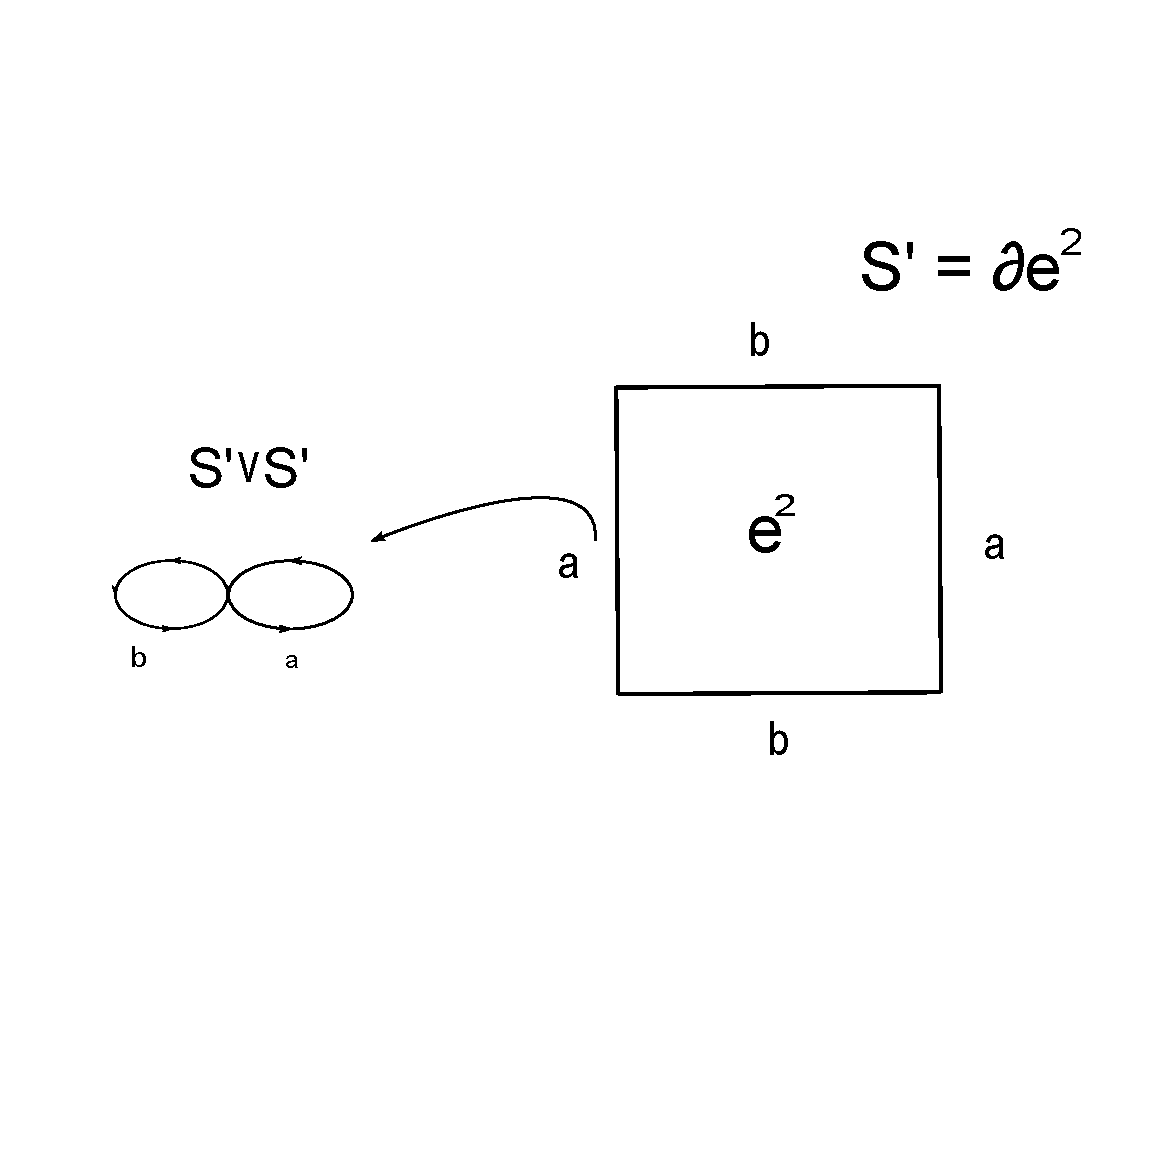
\includegraphics[width=0.3\textwidth]{figures/22.pdf}
%\caption{\small The example $S^1 \times S^1$.}
%\end{wrapfigure}
%\begin{figure}[h!]
%\centering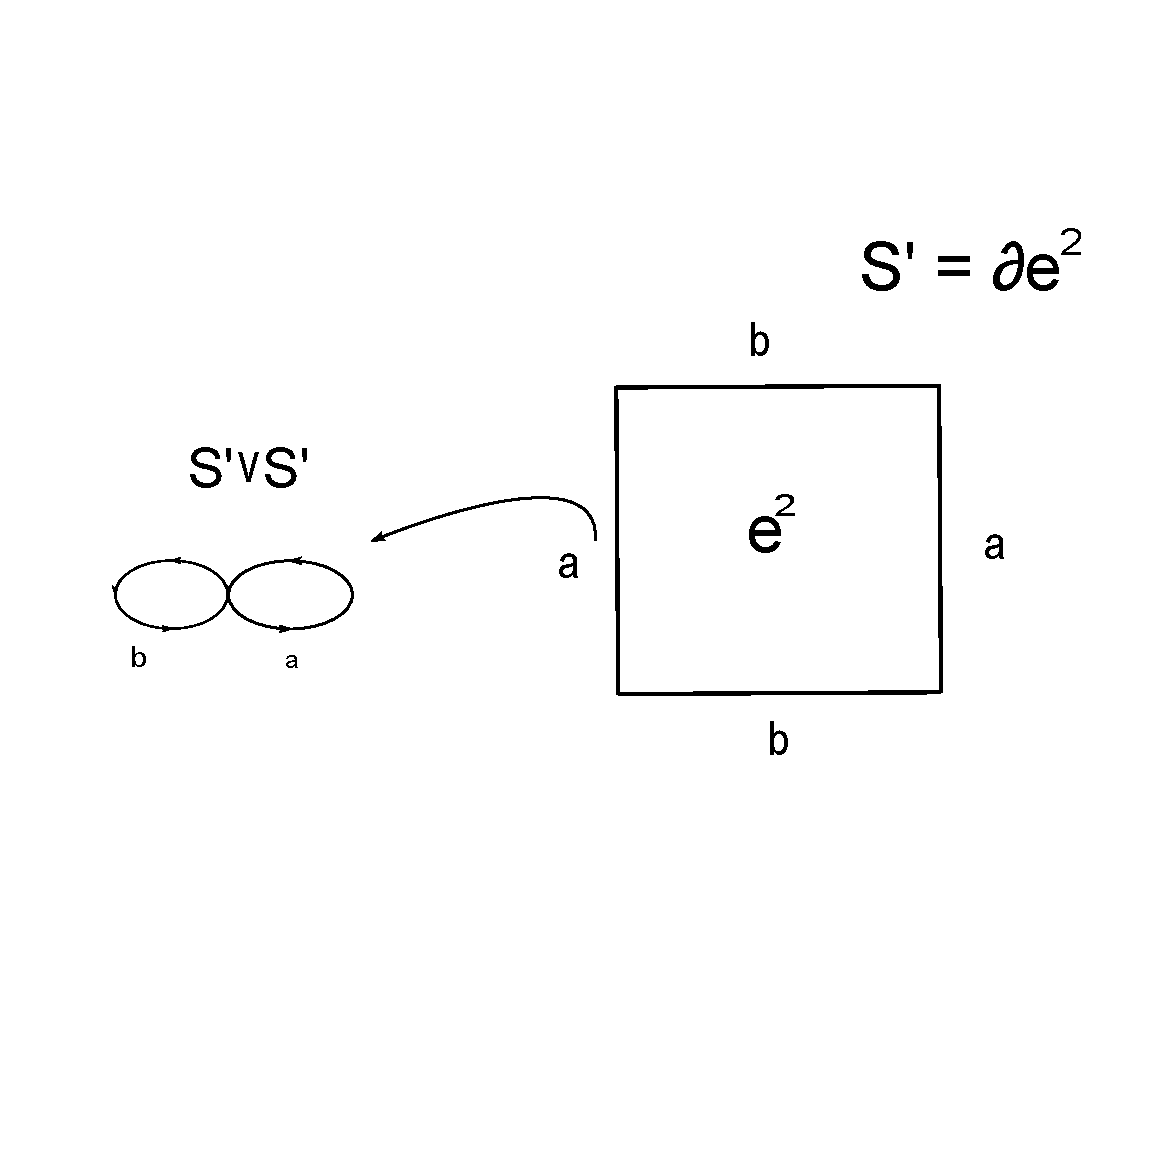
\includegraphics[width=0.3\textwidth]{figures/22.pdf}
%\caption{\small The example $S^1 \times S^1$.}
%\end{figure}
Another way to think about $W$ is as follows. $S^{p}\times S^{q}$ is a quotient of $e^p\times e^q$, under the product of the quotient maps $\pi:e^p\to S^p$ and $\pi':e^q\to S^q$ given by collapsing boundaries. In fact, this quotient map is part of a pushout diagram (drawn on the left):
\[\ \ \ \ \xymatrix{
e^p\times e^q\ar[r]^{\pi\times\pi'}&S^p\times S^q\\
\makebox[0cm][r]{$S^{p+q-1}=$\,}
\partial(e^p\times e^q)\ar@{^{(}->}[u]\ar[r]^W&S^p\vee S^q\ar@{^{(}->}[u]
}
\raisebox{-.6cm}{\qquad where\qquad}
\xymatrix{
e^p\ar[r]^{\pi\ \ \ }&S^p\vee S^q&e^q\ar[l]_{\ \ \ \pi'}\\
\ar[u]^{\textup{pr}_1}
e^p\times S^{q-1}\ar@{^{(}->}[r]&\partial(e^p\times e^q)\ar[u]^W&\ar@{_{(}->}[l]S^{p-1}\times e^q\ar[u]_{\textup{pr}_2}
}
\]
\ConfusedBox{I could probably put the diagram from my notes here.}
Facts about the Whitehead product: once again, for real proofs, see Whitehead's book.
\begin{enumerate}
\item In the case $p = q = 1$ it is a map $\pi_1 (X) \times \pi_1 (X) \to \pi_1 (X)$, given by $[\alpha, \beta] = \alpha \beta \alpha^{-1} \beta^{-1}$, as can be seen by considering the attaching map of the top cell of the torus. This justifies the bracket notation.  In the case $p = 1$ and $q \ge 1$, this product gives the natural action of $\pi_1 (X)$ on $\pi_q (X)$.
\item Skew commutativity: $[\beta, \alpha] = (-1)^{|\alpha||\beta|}[\alpha, \beta]$.
\item The Jacobi identity: for $\alpha \in \pi_p (X)$, $\beta \in \pi_q (X)$, $\gamma \in \pi_r (X)$:
\[
(-1)^{(r-1)p}[\alpha, [\beta, \gamma]] + (-1)^{(p-1)q}[\gamma, [\alpha, \beta]] + (-1)^{(q-1)r}[\beta, [\gamma, \alpha]] = 0
.\]
\item Interaction with the Hurewicz map.  One way to straighten out the degree shift is to write all the homotopy groups in terms of $\Loops X$; then the Whitehead product is a map $\pi_p (\Loops X) \times \pi_q (\Loops X) \to \pi_{p+q} (\Loops X)$.  On the other hand there is the Hurewicz map $h: \pi_* (\Loops X) \to H_* (\Loops X)$ (and $H_*(\Loops X)$ is a noncommutative algebra with Pontryagin product). Then $h([\alpha, \beta]) = h(\alpha)h(\beta) - h(\beta)h(\alpha)$, i.e., $h$ is a map of Lie algebras.
\item The suspension $\Suspend [\alpha, \beta] = 0$.  We know this fact, that $X \wsum Y \to X \times Y$ splits after one suspension, so that $\Suspend W$ is nullhomotopic.
\item If $X$ is an H-space, then $[\alpha, \beta] = 0$.  This follows from the commutative diagram
\begin{diagram}[height=2em]
S^{p+q-1} & \rTo^W & S^p \wsum S^q & \rTo^{\alpha \wsum \beta} & X \wsum X & \rTo^\Phi & X \\
& \rdTo & \dTo & & \dTo & \ruTo_\mu \\
& & S^p \times S^q & \rTo^{\alpha \times \beta} & X \times X.
\end{diagram}
\end{enumerate}

Now consider the Whitehead product in the case $p = q = n$; here the most interesting case is the ``Whitehead square'' $[\alpha, \alpha]$.  It can be computed in terms of its universal example $[\iota_n, \iota_n] = w_n$, where $\iota_n$ is the fundamental class in $\pi_n (S^n)$. That is, for $\alpha\in\pi_p(X)$, $[\alpha,\alpha]\in\pi_{2p-1}(X)$ is the composite $\alpha \circ w_n$:
\[\xymatrix@R=.7cm@C=0cm
{S^{2p-1}\ar[rr]^{w_n}\ar[dr]_{W}&&S^p\ar[rr]^\alpha&&X\\
&S^p\vee S^p\ar[ur]_{\Phi}\ar@{..>}[rr]^{\alpha\vee\alpha}&&X\vee X\ar@{..>}[ur]_{\Phi}
}\]
Now before, we saw that $W$ was part of a pushout square, drawn on the left below. We also have it that $\Phi$ is part of an adjoining pushout square, drawn at the right:
\[\xymatrix{
e^p\times e^p\ar[r]^{\pi\times\pi'}&S^p\times S^p\ar[r]&J_2(S^p)\\
\makebox[0cm][r]{$S^{2p-1}=$\,}
\partial(e^p\times e^p)\ar@{^{(}->}[u]\ar[r]^W&S^p\vee S^p\ar@{^{(}->}[u]\ar[r]^\Phi &S^p\ar[u]
}\]
Now the outer square is a pushout diagram, and the inclusion of $S^{2p-1}$ in the contractible space $e^p\times e^p$ is a cofibration, so that $J_2(S^n)$ is the mapping cone $C(w_n)$.
%But this all means that the mapping cone $C(W_n) = J_2 S^n$, the second filtration of the free monoid on $S^n$, $JS^N$, from the James construction.

Now $w_n \in \pi_{2n-1} (S^n)$ so we should compute its Hopf invariant, and the inclusion $J_2(S^n)\hookrightarrow J(S^n)\simeq\Omega S^{n+1}$  induces an isomorphism on cohomology algebras up to degree $2n$.\footnote{Recall that after one suspension, $J_2(S^n)$ splits as $\Sigma J_2(S^n)=\bigvee_{\!k\leq2}S^{nk+1}$, compatibly with the splitting $\Sigma J_2(S^n)=\bigvee_{\!k}S^{nk+1}$. In particular, the inclusion $J_2(S^n)\to J(S^n)$ is an isomorphism on homology and cohomology up to degee $2n$.\label{Fottnoteofold}} Moreover, % and we already have a good start since we know that $C W_n = J_2 S^n$.  Now from the James construction we know that $J_2 S^n \into \Loops S^{n+1}$, and moreover
\[
H^* (\Loops S^{n+1} )\cong \begin{cases} \Gamma[x_1], & \hbox{$n$ even}, \\ E[x_1] \otimes \Gamma[x_2], & \hbox{$n$ odd},\end{cases}
\raisebox{-.0cm}{\ \ \  which shows that\ \ \ }
H (w_n)= \begin{cases}2, & \hbox{$n$ even}, \\ 0, & \hbox{$n$ odd}.\end{cases}
\]
Well, this is pretty nice, in fact it's pretty amazing: what we've done is look at
\[
\pi_{2n-1} (S^n) \stackrel{h}{\to} \pi_{2n-1}(S^{2n-1}) = \Z
\]
and show that the image contains $2\Z$ is $n$ is even. Thus there is a short exact sequence
\[0\to \ker (h)\to\pi_{2n-1}(S^n)\to\left(\im(h)\cong\Z\right)\to0.\]
As $\Z$ is free, this sequence splits, and $\pi_{2n-1}(S^n)\simeq\ker(h)\oplus\Z$. This, and $\pi_n (S^n) = \Z$ are in fact the only free abelian summands in higher homotopy groups!  Now if you're away from $2$, $2$ is as good as one; in other words a corollary of the above and our calculation of $H^* (\Loops S^{n+1})$ is:
\ConfusedBox{\textbf{Don't we also need to be away from all the other primes, so that the EHP sequence is a fiber sequence? I.e. Doesn't this need to be done rationally?} Wait, maybe not! `the above' may simply refer to what's a couple of lines above this box.}
\begin{cor}
For $n$ even, away from $2$, $\Loops S^n \simeq S^{n-1} \times \Loops S^{2n-1}$, i.e.:
\[\pi_{*+1} (S^n) \otimes \Z[\nicefrac{1}{2}] \cong (\pi_* (S^{n-1}) \oplus \pi_{*+1} (S^{2n-1})) \otimes \Z[\nicefrac{1}{2}].\]
\end{cor}
Now remember the $h$ map appeared in the long exact sequence
\[\xymatrix{
\pi_{k+n} (S^n) \ar[r]^{e\ \ \ } & \pi_{k+n+1} (S^{n+1})\ar[r]^h&\pi_{k+n+1} (S^{2n+1}) \\
}\]
as the obstruction to desuspending a class in $\pi_{k+n+1} (S^{n+1})$, so that:
\begin{cor}
For $n$ odd, $w_{n-1} \in \pi_{2n-3} (S^{n-1})$ doesn't desuspend, and for $n$ even it desuspends at least once.
\end{cor}
Now $w_{n-1}$ might desuspend more times; you might ask where  it was ``born'' in the sequence
%\[
%\cdots \stackrel{e}{\to} \pi_{k+n} S^n \stackrel{e}{\to} \pi_{k+n+1} S^{n+1} \stackrel{e}{\to} \pi_{k+n+2} S^{n+2} \stackrel{e}{\to} \cdots
%\]
\[\xymatrix{
\cdots \ar[r]&\pi_{2n-6}(S^{n-4})\ar[r]^e&\pi_{2n-5}(S^{n-3})\ar[r]^e&\pi_{2n-4}(S^{n-2})\ar[r]^e&\pi_{2n-3}(S^{n-1})
}\]
And here we see the (as yet) mysterious rebirth of the vector field problem:
\begin{thm}
$w_{n-1} \in \pi_{2n-3} (S^{n-1})$ desuspends to an element in $\pi_{2n-\rho(n)-2}(S^{n-\rho(n)})$ and no further. That is, $w_{n-1}$ desuspends exactly $\rho(n)-1$ times.\footnote{Recall that $\rho(n)$ was the number from the vector field problem (see lecture \ref{IntroductionToVectorFieldsOnSpheres}):
$
\begin{array}{c|cccccccc}
n & 1 & 2 & 4 & 8 & 16 & 32 & 64 & \cdots \\
\hline
\rho(n) & 1 & 2 & 4 & 8 & 9 & 10 & 12 & \cdots
\end{array}
$}
\end{thm}
Now in order to prove this theorem, we have to relate $w_n$ to the EHP sequence; here's one way:
\begin{thm} The Whitehead square factors as:
\begin{diagram}[height=2em]
S^{2n-1} & \rTo^{e^2} & \Loops^2 S^{2n+1} \\
& \rdTo_{\pm w_n} & \dTo>p \\
& & S^n
\end{diagram}
In particular, under $p:\pi_k (S^{2n+1}) \to \pi_{k-2} (S^n)$ we have $e^2 \alpha\longmapsto \pm w_n \circ \alpha$ \textup{(}for any $\alpha\in\pi_{k-2}(S^{2n-1})$\textup{)}.  This is why the $p$ map is called the ``Whitehead product''.\footnote{However, the behavior of $p$ on a class which is not a double suspension is more erratic.}
\end{thm}
\begin{proof}
Starting with the undecorated arrows in the following diagram, we obtain the wavy arrow since $e\circ w_n$ is null, and the dotted arrow by exactness of  $\xymatrix{\pi_{2n+1}(S^{2n+1})\ar[r]^{\ \ p}&\pi_{2n-1}(S^n)\ar[r]^e&\pi_{2n}(S^{n+1})}$:
\[\xymatrix{
\ar@{..>}[d]S^{2n-1}  \ar[r]^{w_n} & S^n \ar[r]\ar@{=}[d] & C(w_n)\ar@{~>}[d] \\
\Loops^2 S^{2n+1} \ar[r]^{\ \ \ p} & S^n \ar[r]^{e\ \ } & \Loops S^{n+1}
}\]
All we need to show is that the dotted map is $\pm e^2$. By the Hurewicz theorem, it is enough to show that it induces an epimorphism on $H_{2n-1}$. This follows from the diagram
\[\xymatrix{
\widetilde H_{2n} (C (w_n)) \ar[r]^{(1)}_\cong & \widetilde H_{2n} (\Loops S^{n+1}) \\
H_{2n}(S^n, w_n (S^{2n-1})) \ar[r]
\ar[u]^{\cong}\ar[d]_\cong^\partial
& H_{2n}(S^n, p(\Loops^2 S^{2n+1}) )
\ar[u]^{\cong}_{(2)}\ar[d]_\cong^\partial
\\
H_{2n-1} (S^{2n-1}) \ar@{..>}[r] & H_{2n-1} (\Loops^2 S^{2n+1})
}\]
if we verify the isomorphisms (1) and (2).  (1) is the fact we already showed in a previous footnote.$^\text{\ref{Fottnoteofold}}$  (2) follows from the following argument involving the spectral sequence of the fibration $\Loops^2 S^{2n+1} \to S^n \to \Loops S^{n+1}$. For ease of reading, write $F\to E\to B$ for the three terms of this fibration. Then the transgression $E^{2n}_{2n,0}\to E^{2n}_{0,2n-1}$ must be an isomorphism, however, there can be no other nonzero differentials in or out of $E_{2n,0}$ and $E_{0,2n-1}$. Now the following diagram defines the transgression:
\[\xymatrix{
H_{2n-1}(F)&\ar[l]H_{2n}(E,F)\ar[r]^{(2)}&H_{2n}(B,*)&%\ar[r]& &&%H^n(\Omega B)\ar@{=}[r]&H^{n+1}(\Sigma\Omega B)&\ar[l]
H_{2n}(B)\ar[l]
}\]
If (2) were not an isomorphism, then the transgression could not be either.
\end{proof}
One consequence of this is
\begin{cor}
$\iota_{2n+1} \mapsto \pm w_n$ under $p:\pi_{2n+1}(S^{2n+1})\to\pi_{2n-1}(S^n)$.
\end{cor}
And so we get
\begin{thm}[G.\ Whitehead]
The kernel of $\xymatrix{\pi_{2n-1}(S^n)\ar[r]^e&\pi_{2n}(S^{n+1})}$\!\! is
%
%In the exact sequence
%$\xymatrix{\pi_{2n+1}(S^{2n+1})\ar[r]^{\ p}&\pi_{2n-1}(S^n)\ar[r]^e&\pi_{2n}(S^{n+1})}$\!,
\[
\ker(e) = \begin{cases} 0 & \hbox{when $n = 1, 3, 7$} \\ \Z_2 \langle w_n \rangle & \hbox{$n$ odd, $n\neq1,3,7$} \\ \Z \langle w_n \rangle & \hbox{$n$ even}. \end{cases}
\]
\end{thm}
\begin{proof}
We'll focus on the excerpt $\xymatrix{\pi_{2n+1}(S^{n+1})\ar[r]^{h\ }&\pi_{2n+1}(S^{2n+1})\ar[r]^{\ p}&\pi_{2n-1}(S^n)\ar[r]^e&\pi_{2n}(S^{n+1})}$. We can describe $\ker(e)=\im(p)$ as the subgroup generated by $\pm p(\imath_{2n+1})=w_n$.

When $n=1,3,7$, there is an element of Hopf invariant one in $\pi_{2n+1}(S^{n+1})$, so that $h$ is surjective, and $p=0$. In particular, $w_n=0$.

When $n\neq1,3,7$ is odd, there is an element of Hopf invariant two in $\pi_{2n+1}(S^{n+1})$, but no element of Hopf invariant one, so that $\im(h)$ has index two in $\pi_{2n+1}(S^{2n+1})$.

When $n$ is even, $w_n$ has hopf invariant two, and so has infinite order.
\end{proof}

OK, now we want to address the desuspension problem, and in order to do that we'll link up all the EHP sequences, I mean, here they are:
\begin{diagram}[height=2em]
S^n & \rTo^e & \Loops S^{n+1} & \rTo^h & \Loops S^{2n+1};
\end{diagram}
apply $\Loops^n$ to get
\begin{diagram}[height=2em]
\Loops^n S^n & \rTo^e & \Loops^{n+1} S^{n+1} & \rTo^h & \Loops^{n+1} S^{2n+1}.
\end{diagram}
Now these link together:
\begin{diagram}[height=2em]
\ptspace & \rTo^e & \Loops S^1 & \rTo^e & \Loops^2 S^2 & \rTo^e & \Loops^3 S^3 & \rTo^e & \cdots & \rTo \bigcup \Loops^n S^n = QS^0 \\
& & \dTo>h & & \dTo>h & & \dTo>h \\
& & \Loops S^1 & & \Loops^2 S^3 & & \Loops^3 S^5,
\end{diagram}
Here, $e:\Omega^{n}S^{n}\to\Omega^{n+1} S^{n+1}$ can be viewed as the
$n$-fold looping of the inclusion of the straight loops $S^{n}\to\Omega S^{n+1}$. In particular, each $e$ realises the suspension homomorphism on homotopy. Moreover, $QS^0$ is given the quotient (a.k.a.\ direct limit) topology, and as such (as $S^k$ is compact):
\[\pi_k(QS^0)=[S^k,\varinjlim\Omega^n S^n]=\varinjlim[S^k,\Omega^n S^n]=\varinjlim\pi_{k+n}(S^n)=\Pi_k.\]
We also note that the map $\pi_k(\Omega^n S^n)\to\Pi_k$ induced by mapping $\Omega^n S^n\to QS^0$ is the stabilisation map.

In particular, this sequence has filtered the stable homotopy groups of spheres by unstable homotopy groups.  But each leg is a fibration, and the corners match, so if you apply homotopy something wonderful happens: you get a sequence of exact triangles whose ends match up (the maps $p$ have degree $-1$ on $\pi_*$).


\begin{diagram}[height=2em]
\pi_*(\ptspace) & \rTo & \pi_* (\Loops S^1) & \rTo^e & \pi_* (\Loops^2 S^2) & \rTo^e & \pi_* (\Loops^3 S^3) & \rTo & \cdots&\rTo&\Pi_* \\
& & \dTo & \luTo_p & \dTo>{h} & \luTo_p & \dTo>{h} \\
& & \pi_* (\Loops S^1) & & \pi_* (\Loops^2 S^3) & & \pi_* (\Loops^3 S^5),
\end{diagram}
This is an \emph{exact couple}, so you get a spectral sequence converging to $\pi_* (Q S^0)=\Pi_*$, whose $E_1$ page consists of the bottom line of the above diagram:
\[
E^1_{s, t} = \pi_{s+t}(\Loops^{s+1} S^{2s+1}) = \pi_{2s+1+t} (S^{2s+1})
\]
so the columns of the spectral sequence are homotopy groups of odd spheres.  So here it is:
\[\textsc{Draw me, please.}\]
The differentials $d_r: E^r_{s, t} \to E^r_{s-r, t+r-1}$, of total degree $-1$, are like the differentials in the usual homology spectral sequence. They are `defined' by the `formula' $d_r=he^{-(r-1)}p$, that is:
\[\xymatrix{
\pi_{s+t-1}(\Omega^{s-r+1}S^{s-r+1})\ar[rr]^{\qquad r-1}_{\qquad\text{desuspensions}}\ar[d]^h&&
\pi_{s+t-1}(\Omega^s S^s)\\
\makebox[0cm][r]{$E^1_{s-r,t+r-1}=$\,}\pi_{s+t-1}(\Omega^{s-r+1}S^{2s-2r+1})&&&\ar[ul]_p\makebox[0cm][r]{$E^1_{s,t}=$\,}
\pi_{s+t}(\Omega^{s+1}S^{2s+1})
}\]
Of course, this `definition' does not make sense on the groups $E^1_{s,t}$. Instead, it makes sense on the subquotients $E^r_{s,t}$ of the $E^1_{s,t}$. In fact, we may define, for $0\leq r\leq\infty$:\footnote{One should check that this definition gives $E^1_{s,t}=\pi_{s+t}(\Omega^{s+1}S^{2s+1})$, and that can be made to make sense when $r=\infty$. By convention, we regard $\Omega^n S^n$ to be the one point space when $n<0$.}
\begin{alignat*}{2}
Z_{st}^r:=&\left\{x\in \pi_{s+t}(\Omega^{s+1}S^{2s+1})\ \middle|\ p(x)\in\im(e^{r})\right\}\\
=&\left\{x\ \middle|\ \text{$p(x)\in\pi_{s+t-1}(\Omega^s S^s)$ desuspends to an element of $\pi_{s+t-1}(\Omega^{s-r} S^{s-r})$}\right\}.\\
B_{st}^r:=&\left.h(\ker(e^r))\right.\\
=&\left\{h(y)\ \middle|\ y\in \pi_{s+t}(\Omega^{s+1}S^{s+1}),\ e^r(y)=0\in \pi_{s+t}(\Omega^{s+r+1}S^{s+r+1})\right\}\\
=&\left\{\text{James-Hopf invariants $h(y)$ of classes $y$ vanishing after $r$ suspensions}\right\}.\\
E_{st}^{r+1}:=&\left.Z_{st}^r/B_{st}^r.\right.
\end{alignat*}
Given this definition, and the above definition of the differentials $d_r$, it is an exercise in diagram chasing to check that we have given the data of a spectral sequence.

For each $s,t\geq0$, let $e_{st}:\pi_{s+t}(\Loops^{s+1} S^{s+1})\to \Pi_{s+t}$ be the stabilisation homomorphism. Then there is an increasing filtration on $\Pi_{s+t}$ defined by $F_{s}\Pi_{s+t}:=\im(e_{st})$. Let $\Gr_{st}$ be the subquotient $F_{s}\Pi_{s+t}/F_{s-1}\Pi_{s+t}$:
%\[\Gr_{st}:=F_{s}h_{s+t}(E)/F_{s-1}h_{s+t}(E).\]
%With this notation:
\[
\Gr_{st}:=\frac{\im\bigl(\pi_{s+t}(\Omega^{s+1} S^{s+1})\rightarrow \Pi_{s+t}\bigr)}{\im\bigl(\pi_{s+t}(\Omega^s S^{s})\rightarrow \Pi_{s+t}\bigr)}.\text{\ \ \ Note also:\ \ }
Z_{st}^\infty=
h(\pi_{s+t}(\Omega^{s+1}S^{s+1}));\text{\ and\ }
B_{st}^\infty=h(\ker (e_{st})).
\]
The spectral sequence converges to $\Pi_{s+t}$, in that there are isomorphisms $E_{st}^\infty\to \Gr_{st}$ defined by:
\[[h(y)]\longmapsto [e_{st}(y)]\text{ for $y\in \pi_{s+t}(\Omega^{s+1}S^{s+1})$}\]
Now if $z\in F_s\Pi_{s+t}$, then there is some $\overline z\in \pi_{s+t}(\Omega^{s+1} S^{s+1})$ such that $e_{st}(\overline z)=z$. The inverse isomorphism $\Gr_{st}\to E_{st}^\infty$ is then given by:
\[[z]\longmapsto [h(\overline z)].\]
That is to say the following. Given an element $z\in\Pi_n$ in the stable $n$-stem, desuspend $z$ as far as possible to an element of $\overline z\in\pi_{n}(\Omega^{s+1}S^{s+1})$, then $h(\overline z)\in \pi_{n}(\Omega^{s+1}S^{2s+1})=:E^1_{s,n-s}$ is a permanent cycle detecting $z$. One could summarise by stating that $z$ is recorded by the James-Hopf invariant of a maximal desuspension.

Now an obvious question is this: if you think of a spectral sequence as a way of computing the $E^\infty$ term from the $E^1$ term, well, why isn't this game hopeless?  We have a spectral sequence converging to stable homotopy whose input is \emph{unstable} homotopy, which could very well be more difficult to compute.  But one really neat feature of this game is that in
\begin{diagram}[height=2em]
\ptspace & \rTo & \Loops S^1 & \rTo & \Loops^2 S^2 & \rTo & \Loops^3 S^3 & \rEqualto & \Loops^3 S^3 & \rEqualto & \Loops^3 S^3 & \cdots \\
& & \dTo & & \dTo & & \dTo & & \dTo & & \dTo \\
 & &\Loops^1 S^1& & \Loops^2 S^3 & & \Loops^3 S^5 & & 0 & & 0
\end{diagram}
we can just \emph{stop} the exact couple anywhere, and get an identical spectral sequence to the one we just saw except that we'll have zeroes in the columns beyond where we stop; otherwise, the picture is the same.  And the spectral sequence we get will converge to the homotopy of the sphere in the last column; in the case above, for example, $\pi_* (\Loops^3 S^3)$.  So actually we have a whole family of spectral sequences converging to the input of our original spectral sequence.

Well, that still doesn't sound very good, except that you can play all of these facts off each other and often you can get pretty far.  For example, let's look at $d_1$, the composite:
\[\xymatrix{
\makebox[0cm][r]{$E^1_{s,t}=$\,}
\pi_{s+t}(\Omega^{s+1}S^{2s+1})\ar[r]^{\ p}&\pi_{s+t-1}(\Omega^s S^s)\ar[r]^{h\ \ }&\pi_{s+t-1}(\Omega^{s}S^{2s-1})\makebox[0cm][l]{\,$=E^1_{s-1,t}$}
}\]
Well, on the bottom row (when $t=0$), $E^1_{s,t}$ and $E^1_{s-1,t}$ are both isomorphic to the integers. We only need to know what happens to the generator $\imath_{2s+1}$:
\[\imath_{2s+1}=e^2\imath_{2s-1}\overset{p}{\longmapsto}\pm \imath_{2s-1}\circ w_{s}=w_s\overset{h}{\longmapsto} \pm h(w_s)=\begin{cases}2\imath_{2s-1},&\text{$s$ even,}\\0,&\text{$s$ odd.}\end{cases}\]
Thus we have calculated the $d_1$ differential on the bottom row.
% we only need to know what happens to $\iota_{2s+1} \in \pi_s \Loops^{s+1} S^{2s+1} = \pi_{2s+1} S^{2s+1} = \Z \langle \iota_{2s+1} \rangle$.  But we already computed that considering that $\iota_{2s+1} \in \pi_{2s-1} \Loops^2 S^{2s+1}$, we get $p(\iota_{2s-1}) = w_s$, $p: \pi_{2s-1} \Loops^2 S^{2s+1} \to \pi_{2s-1} S^s$.  $d_1(\iota_{2s+1})$ is thus $h(w_s) \in \pi_{2s-1} (S^{2s-1})$, which is $\pm 2 \iota_{2s-1}$ when $s$ is even or $0$ when $s$ is odd.  So in fact we can write INKSCAPE

But we can get more out of this information: notice that this is the \emph{only} differential \emph{into} the bottom row, and the only differential \emph{out} of the bottom row for columns $s \le 2$.  So we can truncate this spectral sequence and nothing more happens. This spectral sequence computes $\pi_* (\Loops^3 S^3)$, so we have found that $\pi_4 (S^3) \cong \Z_2$.  But by the Freudenthal theorem, for stem degree $1$, $S^3$ is already in the stable range.  So in fact $\pi_{n+1} (S^n) = \Z_2$ for $n \ge 3$.  And this in turn lets us fill in a whole row of the original spectral sequence.

%\ConfusedBox{
%\textbf{On Repeat:}

%Last time we saw the introduction of the EHP spectral sequence.  Remember the $E^1$ term looked like this: INKSCAPE
Now earlier we claimed that introducing the EHP spectral sequence would help to attack the theorem about desuspending $w_n$.  In order to see why this might be true, let's take a look at how to interpret the differentials in the spectral sequence. Note that this discussion will apply in general to any spectral sequence arising from an exact couple.
Two lessons are of great importance in sorting everything out:
\begin{enumerate}
\item We can truncate the sequence of triangles anywhere we want, obtaining a spectral sequence, compatible in some sense with the first, that converges to the homotopy of a finite sphere. To be explicit, for any $M<\infty$, we have a diagram of fibrations:
\[\xymatrix{
\ptspace\ar[r]&\Omega S^1\ar[d]\ar[r]&\Omega^2 S^2\ar[d]\ar[r]&\Omega^3 S^3\ar[d]\ar@{.>}[rr]&&\Omega^{s+1}S^{s+1}\ar[d]\ar@{.>}[rr]&&\Omega^{M}S^{M}\ar[d]\\
&\Omega S^1&\Omega^2 S^3& \Omega^3S^5&&\Omega^{s+1}S^{2s+1}&&\Omega^{M}S^{2M-1}
}\]
The corresponding spectral sequence has exactly $M$ nonzero columns ($0\leq p <M$), and converges to the stem $\pi_{s+t}(\Omega^{M}S^{M})$ of $S^{M}$. Now $E^1_{st}=0$ for $s\geq M$, and:
\[E_{st}^1=\pi_{s+t}(\Omega^{s+1}S^{2s+1})=\pi_t(\Omega^{2s+1}S^{2s+1})\text{ which is in the stable range when $t< 2s$}.\]

\item The second lesson concerns how an element of $\pi_* (S^M)$ is recorded in the truncated spectral sequence (and therefore in the big spectral sequence if you take $M$ large enough).  Since everything is recorded in terms of its James-Hopf invariant, and this is the obstruction to desuspending an element of $\pi_* (\Loops^M S^M)$, the recipe is
\begin{enumerate}
\item Desuspend as far as possible, and then
\item compute the James-Hopf invariant $h$;
\end{enumerate}
this is the filtration at which a given element appears. In fact, if an element $z$ of $\pi_{s+t}(\Omega^MS^M)$ has a maximal desuspension $\overline z$ in $\pi_{s+t}(\Omega^{s+1}S^{s+1})$, then it is the class of $h(\overline z)$ in $E^{\infty}_{s,t}$ which detects $z$. Of course, when you study this at the $E^1$ level, viewing $h(\overline z)$ as an element of $\pi_{s+t}(\Omega^{s+1}S^{2s+1})$, there is an indeterminancy in the value of $h(\overline z)$ associated with the choice of desuspension $\overline z$ of $z$. Evidently, this indeterminacy is exactly $B_{st}^\infty$, but $B_{st}^\infty$ precisely corresponds to the various differentials coming into the target group from elsewhere.

Now the group $\pi_{s+t}(\Omega^{s+1}S^{2s+1})$ in which $h(\overline z)$ resides lies in the stable range when $t<2s$. So unless the element $z$ can be desuspended sufficiently many times that $t\geq2s$, $h(\overline z)$ is a stable homotopy class of sphere.

Moreover, if $z$ desuspends so few times that $t=0$, (i.e.\ $z\in\pi_s(\Omega^M S^M)$ desuspends to $\pi_s(\Omega^{s+1} S^{s+1})$ and no further\footnote{It must desuspend at least this far, by the Freudenthal suspension theorem! Alternatively, it must desuspend at least this far, as all the groups $E_{st}^1$ with $t<0$ are zero, by the same connectivity considerations which were used to prove the suspension theorem using the EHP long exact sequence.}), then $h(\overline z)$ takes values in $\pi_{s}(\Omega^{s+1}S^{2s+1})=\Z$ (with indeterminacy $B_{s0}^\infty$) As we have seen, $h(\overline z)=\pm H(\overline z)$, where $H$ is the standard Hopf invariant.
%\item When $q$ is $0$, $h_*\sigma$ is an element of the stable $0$-stem, and thus a genuine integer, which happily equals the old-fashioned Hopf invariant. More generally, when $q\leq 2p-2$, $h_*\sigma$ lands in the stable $q$-stem, so terms on the $E^\infty$ page which lie below a line of slope two are recorded by a `Hopf invariant' which lies in a stable homotopy group of spheres.
\end{enumerate}



Now in the $E^1$ context, what do the differentials mean?\footnote{I want to advertise this as a great way to understand how various homotopy groups interact.}  Recall that $d_1 = hp$, $d_2 = he^{-1} p$, $d_3 = he^{-1} e^{-1} p$, and so on.  So a description of the differential $d_r$ is this: take the class in $\pi_* (\Loops^{s+1} S^{2s+1})$, apply $p$; then desuspend $r-1$ times and record the result in the agreed way, that is, by taking the James-Hopf invariant. The collection of the $d_r$ together can be understood as the obstruction to lifting an element of $\pi_*(\Loops^{s+1} S^{2s+1})$ to an element of $\pi_*(\Loops^{s+1} S^{s+1})$ (using the map $h$).

Before we go on, note that this helps explain why this spectral sequence might be useful in studying how far we can desuspend $w_n$. Explicitly, $p(\iota_{2n+1}) = \pm w_n$, so studying how far you can desuspend $w_n$ is the same as looking for the first non-zero differential in the EHP spectral sequence on the fundamental class in $\pi_n (\Loops^{n+1} S^{2n+1})=E^1_{n,0}$.

Now usually when you attack a problem like desuspending a class, a standard approach is to convert the problem to a stable one and hope that things become more cohomological.  Now suspension gives homomorphisms
\[E_{st}^1=\pi_{s+t}(\Omega^{s+1}S^{2s+1})\overset{e^2}{\longrightarrow}\pi_{s+1+t}(\Omega^{s+2}S^{2s+3})=E_{s+1,t}^1\]
which provide a horizontal operation on the EHP spectral sequence which is an isomorphism when $t<2s$.  So there is a line of slope $2$ on the $E^1$ term beneath which the columns are the same and in fact represent stable homotopy.  So this grid maps (via repeated application of the stabilisation map) to a grid whose columns are stable homotopy and the map is an isomorphism below the line of slope 2.  The question is: is this the $E^1$ term of some spectral sequence which is compatible with the first?  Our next goal is to construct this spectral sequence and the map of spectral sequences.  Then we can play off the differentials on either side, and learn about desuspending the Whitehead square.


% >>>
\fi
\BoxedNote{}
